\chapter{Experiments}
\label{chap:methodology}
\label{chap:experiments}

\section{Overarching Methodology}
Several of the following sections are about selecting a CA problem and letting CA-NEAT have a go at solving it.
In these experiments, the same basic configuration of CA-NEAT is used.
The size of the CA neighborhood (equal to the number of CPPN inputs) and the number of cell-states (equal to the number of CPPN outputs) is changed to be appropriate to the problem at hand.
The fitness evaluation function is also custom to every problem.

Otherwise the CA-NEAT parameters are the same across different experiments.
These are listed in Appendix TODO.
%Notably, the mutation weigths are biased towards adding nodes and connections moreso than removing them, leading to the average network size growing over time.

Each experiment consists of 100 independent runs with the same parameters but different initial populations.
All experiments have a population size of 200 individuals and elitism degree of 1.
Each generation-population is segregated into species by NEAT, with selection and reproduction happening within these groups.
\textit{Sigma scaled selection} \cite{hancock-1994} is used to select pairs for reproduction.

During development of the system, a variation of different configurations were tried for different problems.
When deciding on the experiments to collect results from for this paper,
a deliberate choice was made to use the same CPPN-NEAT configuration and as close to the same CA configuration as possible for all problems.
This makes it easier to make comparison between experiments, but means that the settings chosen may favor some experiments over others.

\section{Morphogenesis and Replication of 2D Patterns}
\label{sec:prev_work}
The first class of problems CA-NEAT was tested on was \textit{morphology problems}, in the form of the two related problem of morphogenesis and replication.
The patterns used in these experiments are shown in Figure \ref{fig:patterns}

\begin{figure*}
\centering
\begin{subfigure}[b]{.20\textwidth}
\centering
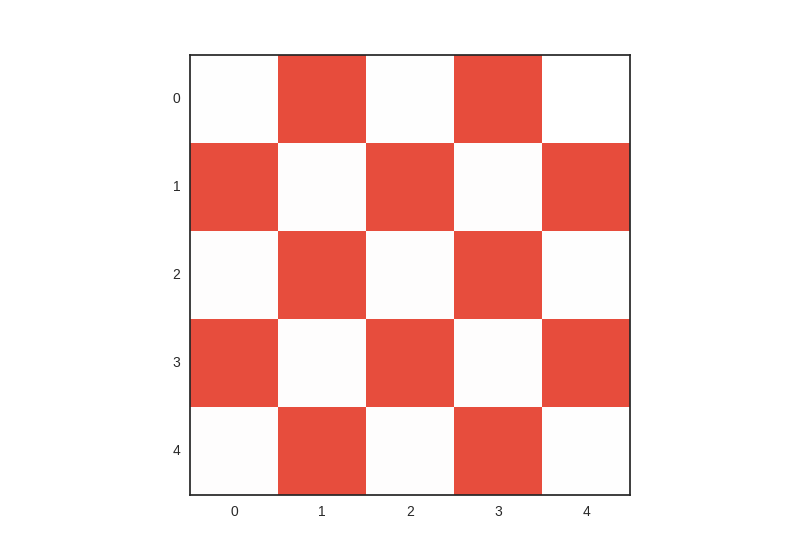
\includegraphics[width=\textwidth]{fig/mosaic}
\caption{5x5 "Mosaic"}
\label{fig:mosaic_pattern}
\end{subfigure}%
\begin{subfigure}[b]{.20\textwidth}
\centering
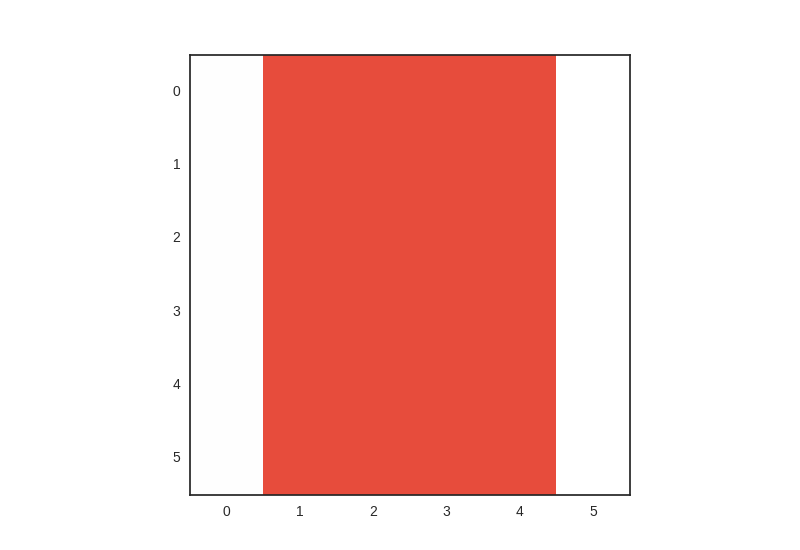
\includegraphics[width=\textwidth]{fig/border}
\caption{6x6 "Border"}
\end{subfigure}%
\begin{subfigure}[b]{.20\textwidth}
\centering
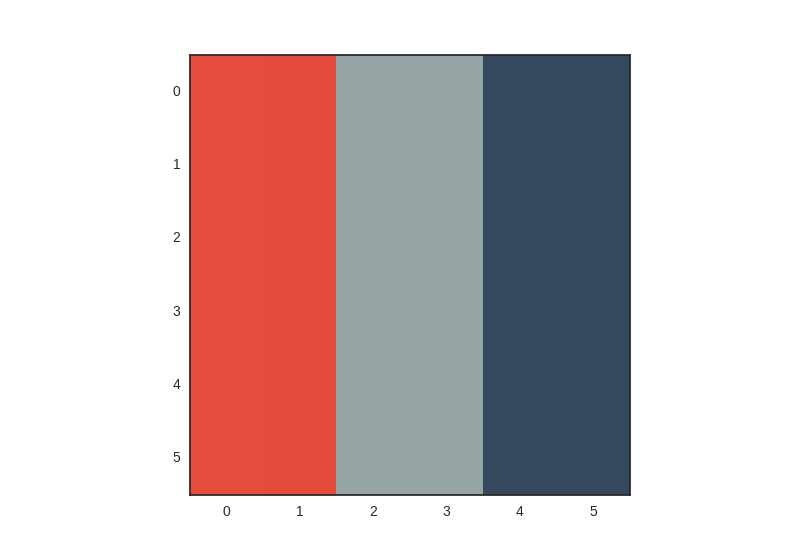
\includegraphics[width=\textwidth]{fig/tricolor}
\caption{6x6 "Tricolor"}
\end{subfigure}%
\begin{subfigure}[b]{.20\textwidth}
\centering
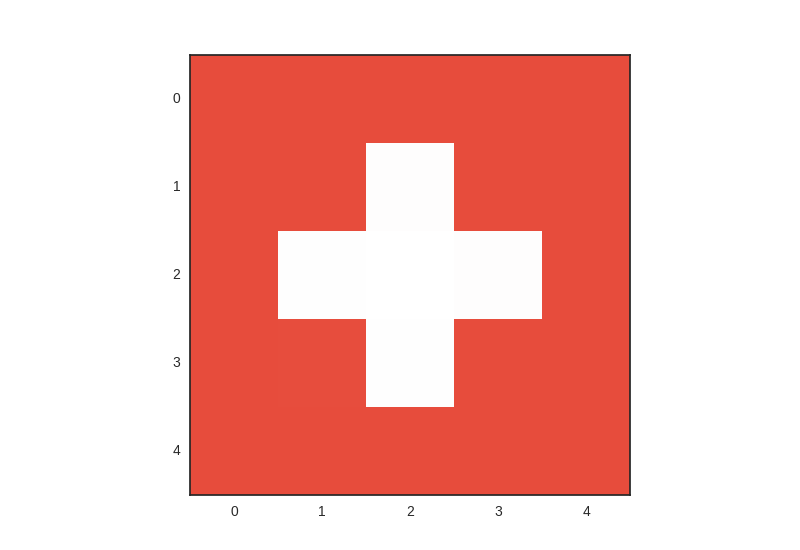
\includegraphics[width=\textwidth]{fig/swiss}
\caption{5x5 "Swiss"}
\end{subfigure}%
\begin{subfigure}[b]{.20\textwidth}
\centering
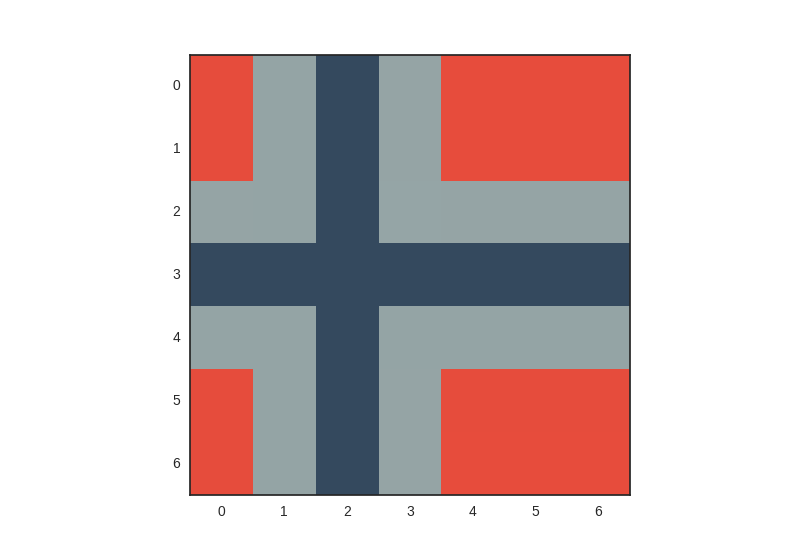
\includegraphics[width=\textwidth]{fig/nordic}
\caption{7x7 "Nordic"}
\end{subfigure}%

\caption{Patterns being investigated for morphogenesis and replication.}
\label{fig:patterns}
\end{figure*}

These are the same problems and patterns as studied in \cite{nichele2014evolutionary}, which used an instruction-based encoding and also tested table-based encoding for comparison.
This allowed the results of \cite{nichele2014evolutionary} to act as a benchmark for testing the CA-NEAT framework during development,
and to make comparisons between the results for analysis.

The experiments in this section were performed and analyzed in the specialization project leading up to this thesis project.
The report from the specialization project was further refined with co-authors Stefano Nichele, Gunnar Tufte and Sebastian Risi to a paper which at the time of writing has been accepted but not yet published in the IEEE Transactions on Cognitive and Developmental Systems.
TODO does mentioning the above go somewhere else?

\subsection{Morphogenesis problems}
\label{sec:morph_problems}
In CA terms, morphogenesis is the construction of a (more) complex pattern from a simple "seed" pattern.
The biological analogy and inspiration is \textit{embryonic development},
with the seed pattern also sometimes called a \textit{zygote}.
Figure \ref{fig:seed} shows the seed patterns used in these experiments.

\begin{figure}
\centering
\begin{subfigure}[b]{.30\columnwidth}
\centering
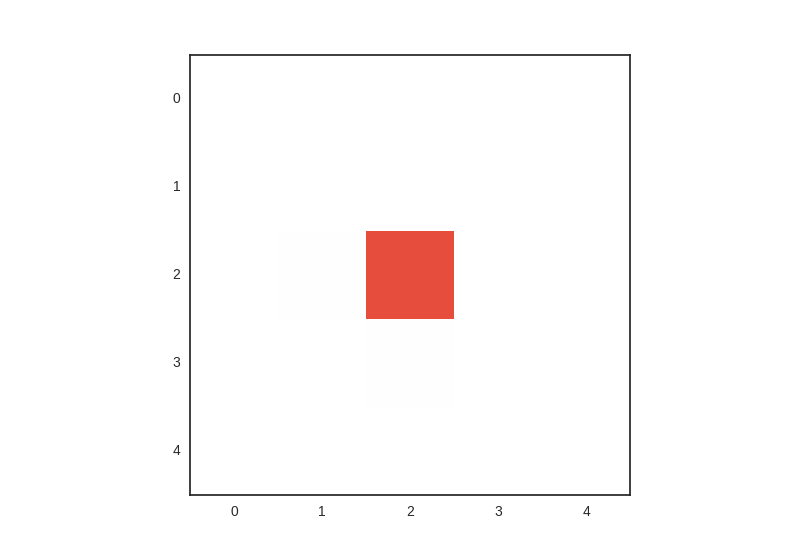
\includegraphics[width=\columnwidth]{fig/seed_5x5}
\caption{5x5}
\end{subfigure}%
\begin{subfigure}[b]{.30\columnwidth}
\centering
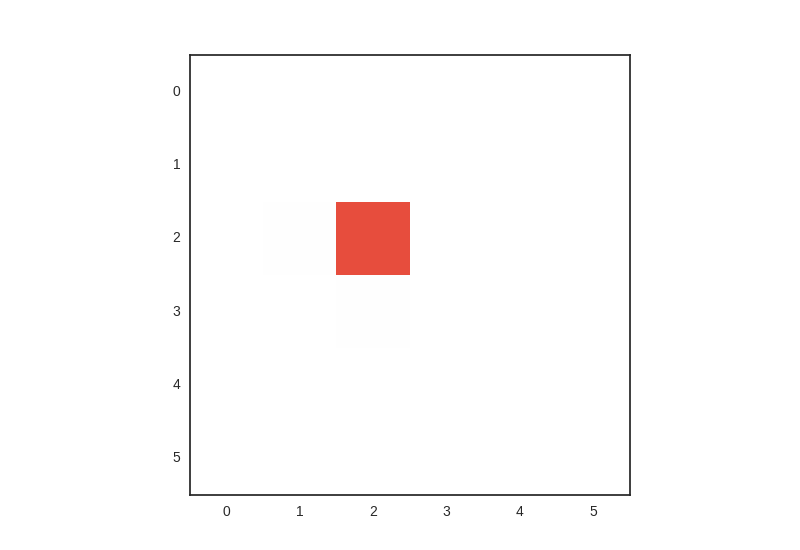
\includegraphics[width=\columnwidth]{fig/seed_6x6}
\caption{6x6}
\end{subfigure}%
\begin{subfigure}[b]{.30\columnwidth}
\centering
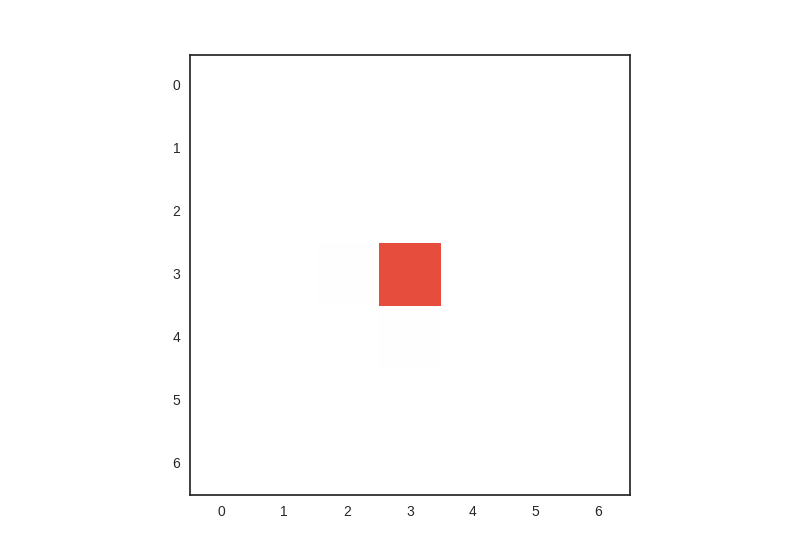
\includegraphics[width=\columnwidth]{fig/seed_7x7}
\caption{7x7}
\end{subfigure}%

\caption
[
    Seed patterns for morphogenesis.
]
{
    Seed patterns for morphogenesis.
    For the 6x6 patterns there is no central cell, so the seed is not symmetric.}
\label{fig:seed}
\end{figure}

The fitness evaluation function used in the morphogenesis experiments consists of the following steps:

\begin{enumerate}
    \item Develop seed pattern for 30 iterations
    \item For each stage
        \begin{enumerate}
            \item Compare cell by cell with  target pattern
            \item Calculate ratio of correct out of total cells
        \end{enumerate}
    \item Pick the highest of the values from step 2
    \item Use function \eqref{eq:redistribute} with value from step 3 as x
\end{enumerate}

\begin{equation}
    \label{eq:redistribute}
    f(x) = x * \frac{e^{5*x}}{e^{5}}
\end{equation}

In cases such as the "Mosaic" pattern (Figure \ref{fig:mosaic_pattern}), a completely dead CA (all cells in the quiescent state) would have a "correct cell" ratio of $0.52$.
Function \eqref{eq:redistribute} is used to reduce the score for such cases, while ensuring that $f(1.0) = 1.0$.

Because every iteration of the CA is counted equally and separately,
the fitness evaluation does not care if the CA becomes stable, enters a cycle, or neither within the 30 allotted iterations.
If the target pattern occurs at any point, that is enough to get a perfect score.

\subsection{Replication problems}
In a CA replication problem, the initial state has some complex pattern present.
The goal is to produce multiple copies of this initial patterns within the allotted time.
The biological analogy of this is cell division and asexual (clonal) reproduction.
For the replication problem the seed pattern is thus one copy of the target pattern in a larger grid.

The fitness evaluation for a replication phenotype is as follows:

\begin{enumerate}
    \item Develop seed pattern for 30 iterations
    \item For each stage
        \begin{enumerate}
            \item For each region of target pattern size
            \begin{enumerate}
                \item Compare cell by cell with  target pattern
                \item Calculate ratio of correct out of total cells
            \end{enumerate}
            \item Pick the highest 3 values from (a)
            \item Multiply any value less than $1.0$ by a penalty factor of $0.9$
            \item Calculate mean of three values
        \end{enumerate}
    \item Pick the highest value from stage (2)
\end{enumerate}

In this case the number of replicas sought is three.
There is no further contribution to the score if there are more than three perfect replicas.
But it follows logically that if one instance can be duplicated once, then each of the duplicates should be able to duplicate again, leading to exponential growth if time and space is not bounded.
Once again a penalty is applied, this time to penalize the contribution from any imperfect replica pattern, hopefully driving the selection pressure towards perfect replication.

Compared to the evaluation of morphogenesis of the same pattern, the replication evaluation is much more computationally expensive.
Therefore it will always take longer to collect results for a replication problem than the same-pattern morphogenesis problem.

\subsection{Cellular Model}
For both morphology problem categories a 2D CA model is used.
For the morphogenesis problem the grid is of fixed size with toroidal border conditions.
For the replication problem the grid is automatically expanding to accommodate growth in any direction.
In theory this means an infinite grid, but since the CA may only iterate 30 times, there is a practical limit to how large it may grow.
For both problem types the Von Neumann neighborhood (Figure \ref{fig:neighborhoods_vn}) is used.

\subsection{Results}
\begin{table*}[h]
    \centering
    \caption[Summary of results of morphology experiments]{
Summary of results.
The metrics shown are the success rate and the mean number of generations until a solution is found, with standard deviation also shown.
In the case of 100\% success rate, the number of generations column shows how many generations it took until the final solution was found.
In the case of less than 100\% success rate, the column shows how many generations were run until the experiment was stopped.
}
\begin{tabular}{lrrrr}
\hline
 Problem              &   Success rate \% &   Mean gens. &   $\sigma$ gens. &   Gens. until stop \\
\hline
Mosaic morphogenesis      &              100 &                1.2 &                 0.4 &                        2 \\
Border morphogenesis      &                1 &              270   &                 0   &                      509 \\
Tricolor morphogenesis    &              100 &               56.5 &               228.8 &                     2189 \\
Swiss morphogenesis       &               76 &              147.7 &               158.9 &                      600 \\
Mosaic replication        &              100 &                4.2 &                10.6 &                       99 \\
Swiss replication         &              100 &                7.7 &                 5   &                       20 \\
Tricolor replication      &               55 &               55.8 &                52.6 &                      200 \\
Nordic replication        &               0  &                  - &                   - &                      200 \\
\hline
\end{tabular}
\label{tbl:results}
\end{table*}

\begin{table}
    \centering
    \caption{Success rate at morphology problems for table-based, instruction-based and CA-NEAT transition functions found by GA.}
    \begin{tabular}{llll}
    \hline
    Problem                & Table-based & Instruction-based & CA-NEAT \\ \hline
    Mosaic morphogenesis   & 55\%        & 98\%              & 100\%   \\
    Swiss morphogenesis    & 23\%        & 100\%             & 76\%    \\
    Border morphogenesis   & 69\%        & 98\%              & 1\%     \\
    Tricolor morphogenesis & 19\%        & 46\%              & 100\%   \\
    Mosaic replication     & 85\%        & 100\%             & 100\%   \\
    Swiss replication      & 1\%         & 100\%             & 100\%   \\
    Tricolor replication   & 8\%         & 100\%             & 45\%    \\
    Nordic replication     & 0\%         & 100\%             & 0\%     \\ \hline
    \end{tabular}
\end{table}

\begin{figure}[t]
\centering
\begin{subfigure}[t]{.45\columnwidth}
\centering
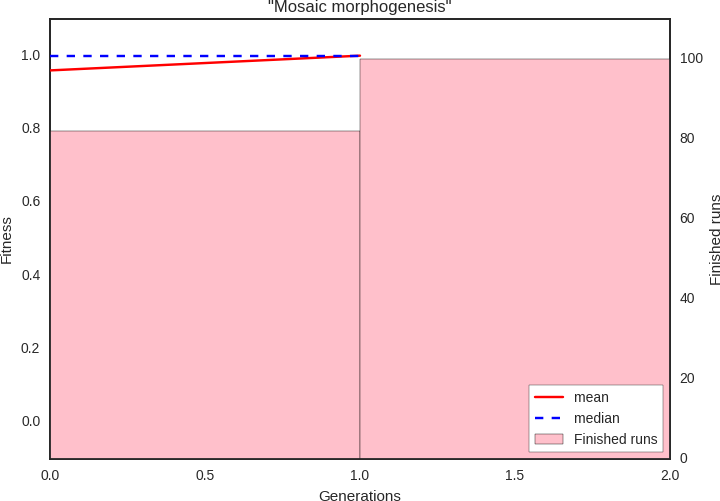
\includegraphics[width=\columnwidth]{fig/generate_mosaic_results}
\caption{Mosaic pattern morphogenesis, all generations.}
\label{fig:generate_mosaic_results}
\end{subfigure}
\begin{subfigure}[t]{.45\columnwidth}
\centering
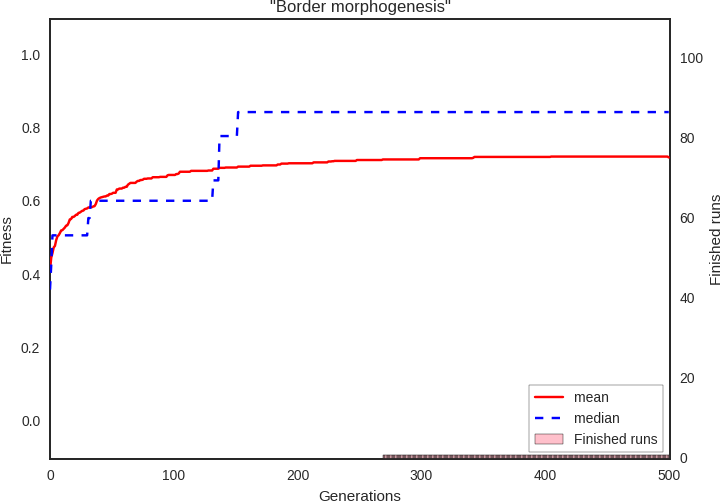
\includegraphics[width=\columnwidth]{fig/generate_border_results}
\caption{Border pattern morphogenesis, 500 first generations.
%The value where the median stabilizes represents the fitness for a solution with one wrong cell.
}
\label{fig:generate_border_results}
\end{subfigure}
\begin{subfigure}[t]{.45\columnwidth}
\centering
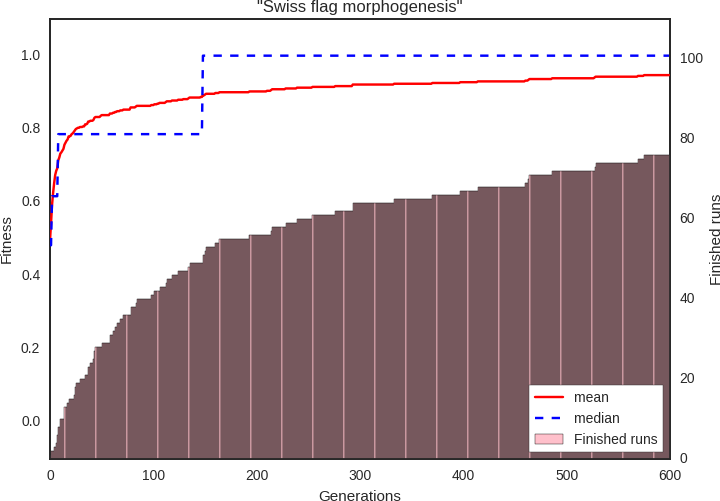
\includegraphics[width=\columnwidth]{fig/generate_swiss_results}
\caption{Swiss flag pattern morphogenesis, 600 first generations.}
\label{fig:generate_swiss_results}
\end{subfigure}
\begin{subfigure}[t]{.45\columnwidth}
\centering
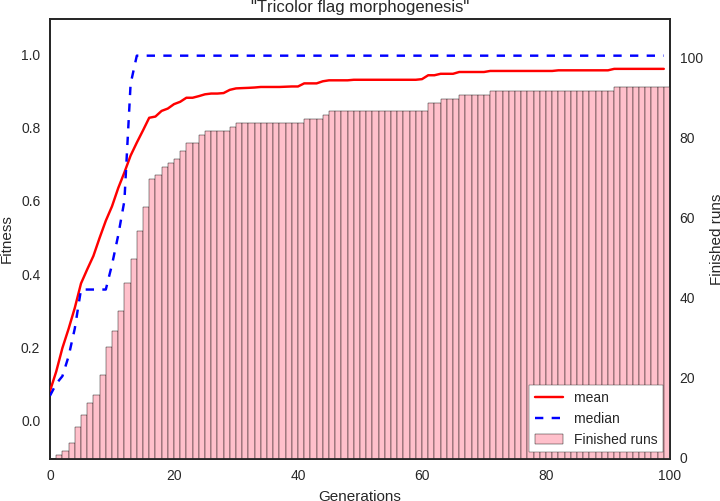
\includegraphics[width=\columnwidth]{fig/generate_tricolor_results}
\caption{Tricolor flag pattern morphogenesis, 100 first generations.}
\label{fig:generate_tricolor_results}
\end{subfigure}
\caption{
    Success rate (cumulative histogram) of the morphogenesis experiments.
    Also shows the mean and median of the max fitness in each run.
    }
\label{fig:morphogenesis_results}
\end{figure}

\begin{figure}[t]
\centering
\begin{subfigure}[t]{.45\columnwidth}
\centering
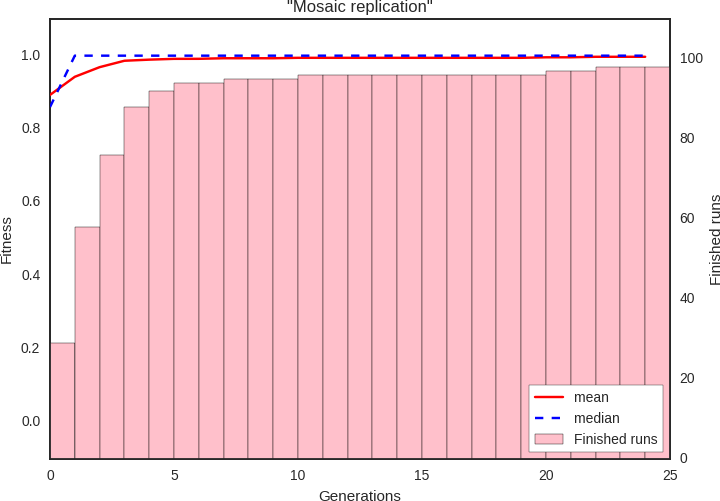
\includegraphics[width=\columnwidth]{fig/replicate_mosaic_results}
\caption{Mosaic pattern replication, 25 first generations.}
\label{fig:replicate_mosaic_results}
\end{subfigure}
\begin{subfigure}[t]{.45\columnwidth}
\centering
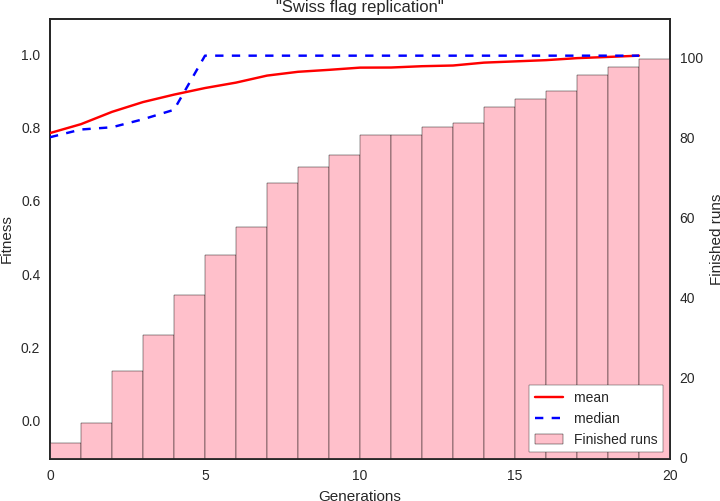
\includegraphics[width=\columnwidth]{fig/replicate_swiss_results}
\caption{Swiss flag pattern replication, all generations.}
\label{fig:replicate_swiss_results}
\end{subfigure}
\begin{subfigure}[t]{.45\columnwidth}
\centering
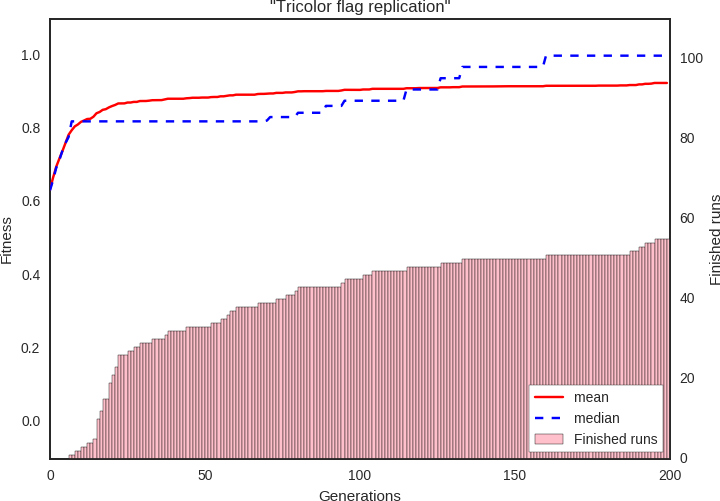
\includegraphics[width=\columnwidth]{fig/replicate_tricolor_results}
\caption{Tricolor flag pattern replication, 200 first generations.}
\label{fig:replicate_tricolor_results}
\end{subfigure}
\begin{subfigure}[t]{.45\columnwidth}
\centering
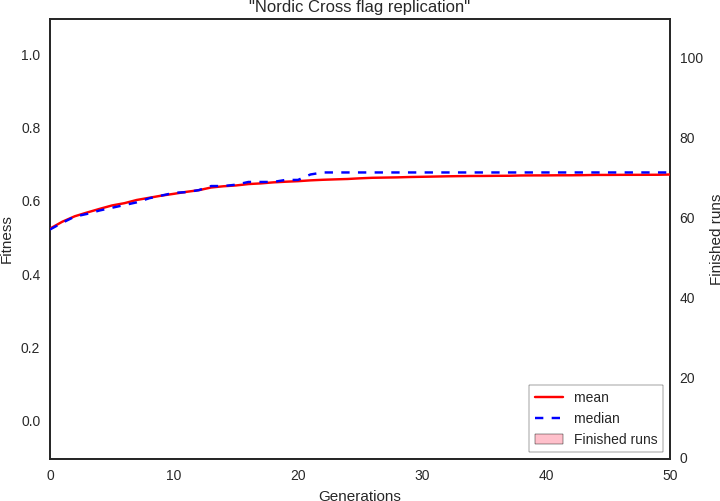
\includegraphics[width=\columnwidth]{fig/replicate_nordic_results}
\caption{Nordic cross pattern replication, 50 first generations.
%Further generations up to 200 did not have any significant change in the mean or median lines.
}
\label{fig:replicate_nordic_results}
\end{subfigure}
\caption{TODO}
\label{fig:replication_results}
\end{figure}

The results of the experiments were varied, with some problems being easily solved with CA-NEAT, some being slowly solved, and some not being consistently solved at all.
Table \ref{tbl:results} summarizes the results in terms of success rate and generations of evolution.
In addition to the varied success rate, there was also a large variation in how many generations of evolution was required to find solutions.
In many cases there was at least one optimal solution among the 20000 individuals generated as part of initial populations.
This means there exists a simple solution consisting of only the input and output layers with connections. 
The most extreme of these cases is the ”Mosaic” morphogenesis where 80 runs complete in the initial generation and the last 20 in the second generation.
This result is understandable, since the pattern has so much symmetry and repetitiveness.
For more complex patterns, more generations of evolution is required in order to bring the success rate nearer 100\%.

It is somewhat surprising which problems are easily solved and which ones are difficult.
The "Swiss" replication is much easier than the "Swiss" morphogenesis,
but the "Tricolor" morphogenesis is easier than the replication of the same pattern.
The fact that the "Border" morphogenesis is much more difficult than the "Tricolor" morphogenesis is not intuitive,
since the "Border" pattern has both fewer colors and one more symmetry.
%Figure \ref{fig:border_almost_correct} shows an example of the close but not perfect patterns CA-NEAT produces for the "Border" morphogenesis.
Perhaps it is the symmetry that is the "trap" which leads to a local maxima,
and the "Tricolor" experiment avoids this,
since symmetry in solutions will not give great scores in that case.
Since the other morphogenesis experiments succeed, and one "Border" solution is found,
there is little reason to suspect that there is any technical error causing poor results.
So the reason must be that the combination of algorithms, problem and parameters cause the problem to be very difficult.
%Further work is required to investigate this.

CA-NEAT does quite well for three out of four replication problems, but fails completely at the "Nordic" replication.
This problem can be expected to be quite difficult, since the pattern is rather complex.
But the instruction-based encoding in \cite{nichele2014evolutionary} did well at the task,
so it is certainly possible to solve the problem with this particular cellular model.
The development of the mean and median lines shown in Figure \ref{fig:replicate_nordic_results} indicate that the evolutionary searches find local maxima from which they can't escape.
%This, along with the "Border" morphogenesis results,
%suggest that the search heuristic may be unsuitable for these problems, and should be reconsidered.

These results were compared with the results of \cite{nichele2014evolutionary}.
It was found that CA-NEAT was able to significantly outperform instruction- and table-based encodings at some problems, while also performing much worse at other problems.
At the morphogenesis tasks, CA-NEAT outperformed the table-based evolution at 3/4 tasks and the instruction-based evolution at 2/4 tasks.
For the replication tasks, CA-NEAT outperformed the table-based evolution at 3/4 tasks and tied at 0\% for the last task.
Instruction-based evolution had a 100\% success rate at all replication tasks.
CA-NEAT equaled this rate at two of the tasks, had some success at one task, and failed completely at the last task.

Figures \ref{fig:tricolor_point_attractor} and \ref{fig:mosaic7} shows visualizations of two results found by evolution.
A larger selection of visualizations is available in the appendix of TODO.

TODO

\begin{figure}
\centering
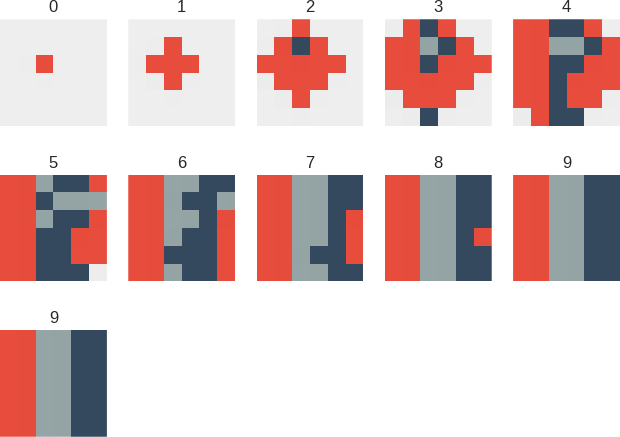
\includegraphics[width=\textwidth, keepaspectratio]{fig/result_figs/generate_tricolor/1}
\caption[A solution to the "Tricolor" morphogenesis]{A solution to the "Tricolor" morphogenesis that finds a point attractor equal to the target pattern.
Most solutions seen did not stabilize like this, but instead found a variety of cycles.}
\label{fig:tricolor_point_attractor}
\end{figure}

\begin{figure}
\centering
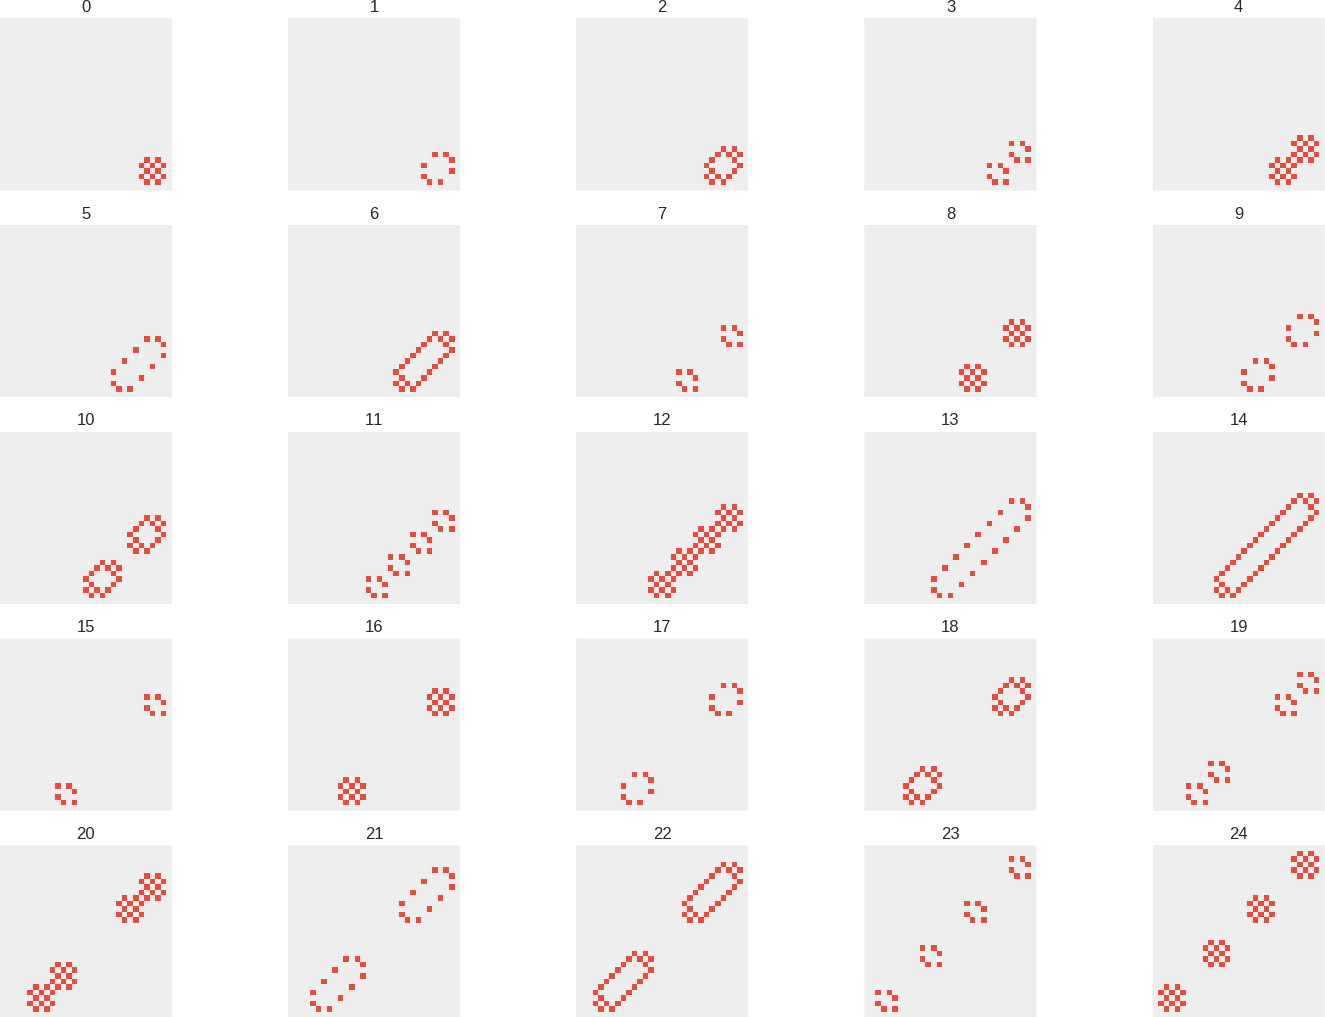
\includegraphics[width=\textwidth, keepaspectratio]{fig/result_figs/replicate_mosaic/7}
\caption[A solution to the "Mosaic" replication]{A solution to the "Mosaic" replication that shows multiple stages of replication.
First the original replicates into two copies. Then each copy tries to replicate, but they interfere with each other and instead return to one copy each, but at a greater distance.
Then they each succeed in replicating, producing four copies total.}
\label{fig:mosaic7}
\end{figure}


\section{2D Morphogenesis With Coordinate Inputs}
\label{sec:morphXY}
Adding environmental information to the CA may make it possible to solve a task that is difficult with only the neighborhood information.
The morphogenesis task makes for a nice test case.
For this experiment, the cellular model is extended to include coordinate information, as described in Section \ref{sec:input_extensions}.
The "Border" and "Nordic" patterns (Figure \ref{fig:patterns}) are targeted in separate experiments.
The "Border" morphogenesis in the previous experiment did not work very well, so it makes for a good comparison.
The "Nordic" pattern is also difficult to generate with the cellular model (TODO because), so it was not attempted in the previous experiment,
but is attempted now.

The quiescent rule is still in place: a cell may not change state if all the neighbors are quiescent, even if the information from the coordinates is available to inform a decision.
The coordinate information is meant to be used in conjunction with the neighborhood information, not to replace it.
If this was not the case, evolution could come up with a CPPN where all the neighborhood inputs were disconnected from the output,
and a static pattern was produced in one time step, like in Figure \ref{fig:cppn}.
That is not a result that we are interested in.

\subsection{Results}

\begin{figure}
\centering
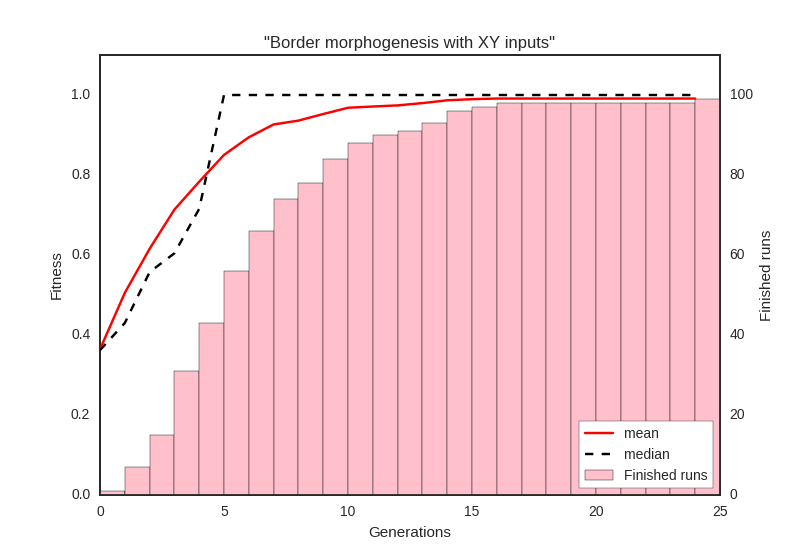
\includegraphics[width=\textwidth, keepaspectratio]{fig/generate_border_extended_results}
\caption{
    TODO
    One trial had yet to succeed when the experiment was stopped at 100 generations.
}
\label{fig:generate_border_extended_result}
\end{figure}


\begin{figure}
\centering
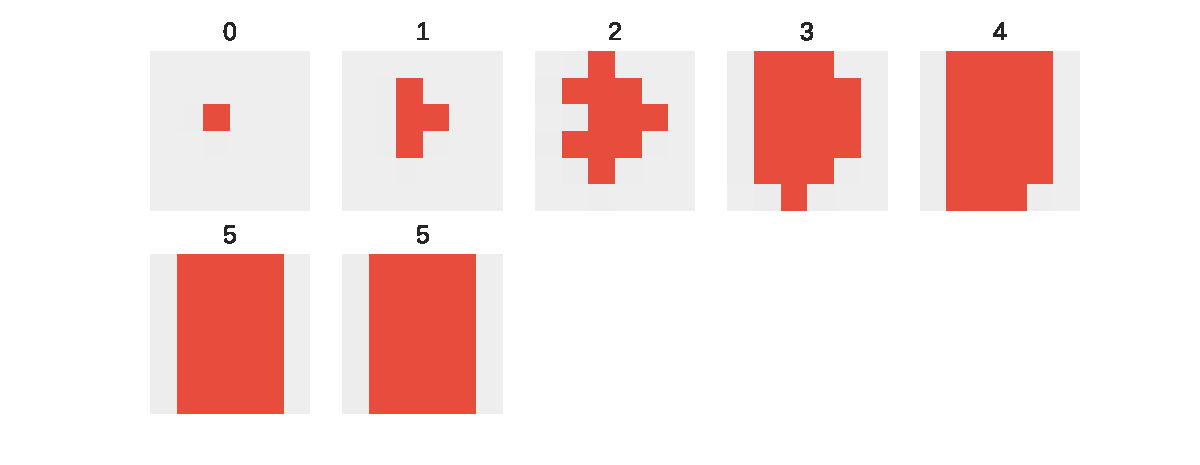
\includegraphics[width=\textwidth, keepaspectratio]{fig/result_figs/border_point_5}
\caption{
    TODO
}
\label{fig:border_point_5}
\end{figure}

TODO

\section{Majority Problem}
The \textit{majority problem} is a problem for 1D binary CA.
It is also called the \textit{density classification task} in literature \cite{mitchell1993revisiting, mitchell1996evolving}.
In this task, the CA should have some arbitrary initial configuration where one "color" (black/white) is more common than the other.
The CA must then figure out which color this is and end up in a point attractor state where all the cells are of this color.
Depending on the initial configuration this can be easy, or very difficult, so finding a general solution that can figure out any initial configuration is difficult.
Even if the majority of the configuration is black, there might be a sub-region that is majority white.
The lack of global overview means that the CA needs to send information around the grid and "negotiate" a consensus about the color.
This problem has been studied extensively with table-based transition functions found by genetic algorithm \cite{mitchell1993revisiting, mitchell1996evolving, mitchell-2001} 

The experiment design here is inspired by the design in TODO cite.

10 initial configurations are created with a specific ratio of black and white cells, but in a random order.
Five are white-dominated and five are black-dominated.
The fitness function tests the rule on each of the configurations and calculates whether the 

\subsection{Results}
TODO


\section{Synchronization Problem}
Another problem for binary 1D CA is the \textit{synchronization problem}.
From some arbitrary initial configuration,
the CA should find its way to a two-step cyclic attractor where all cells share the same state in one timestep,
then all share the other state in the next timestep.
It is thus similar to the majority problem in the way information must be transmitted across the CA in order to coordinate the cells,
but instead of having to "count" cells and landing in a specific point attractor, it finds a cyclic attractor without concern for which of the two states it visits first.

The fitness evaluation function for this experiment is based on the one described in \cite{das1995evolving}, with some modifications.
$K=100$ random initial CA configurations of size $n=49$ are generated from a uniform distribution.
Each candidate solution is first tested on $I=25$ initial configurations.
Each test has a maximum of $2*n$ iterations before being stopped.
If none of the $I$ configurations results in the desired behavior, a fitness of $0.0$ is reported.
If any of the configurations does result in the desired behavior, the candidate is tested on all $K$ configurations.
The fitness reported is then the fraction of configurations that results in the correct behavior.

\subsection{Results}
\begin{table}
\centering
\begin{tabular}{c|c}
Rate & \# \\\hline
0.94 & 1 \\
0.95 & 2 \\
0.96 & 2 \\
0.97 & 65 \\
0.98 & 27 \\
0.99 & 3 \\
1.0 & 0 \\
\end{tabular}
\caption{Distribution of max fitness achieved in 100 independent trials}
\label{tbl:synchronization_training}
\end{table}

Table \ref{tbl:synchronization_training} shows the distribution of the best achieved fitness in the 100 independent trials.
None of the trials achieved 100\% coverage of the configurations, but three trials managed to solve all except one.
95 out of 100 trials achieved 0.97 or greater.
Because of the uniform distribution the initial configurations are sampled from,
it is to be expected that a lot of the configurations are similar in that a behavior that can solve one of them can solve many of them.
It is therefore not surprising to find scores greater than $0.9$ early.
The challenge is to be able to solve all the tricky configurations and get the last few tests right.

The method of fitness evaluation used during evolution does not create an absolute measure of fitness unless the set of tests contains all $2^n$ possible initial configurations.
After the evolution is finished, new test configurations are created to re-assess the performance.
This way the solutions can be tested on different grid sizes as well.
Testing on new configuration of various sizes should give a good indication of how general the solutions found are.

To test the performance of the best of each run,
a sample is selected by picking the top 10 performing individuals from each run.
These 1000 individuals are then categorized by CA behavior (as described in Section \ref{sec:behavior}),
and when duplicates are removed, only 48 distinct behaviors remain.
This set of 48 distinct individuals is designated as "candidates" for best solution, and are subjected to the more extensive testing.

\begin{figure}
\centering
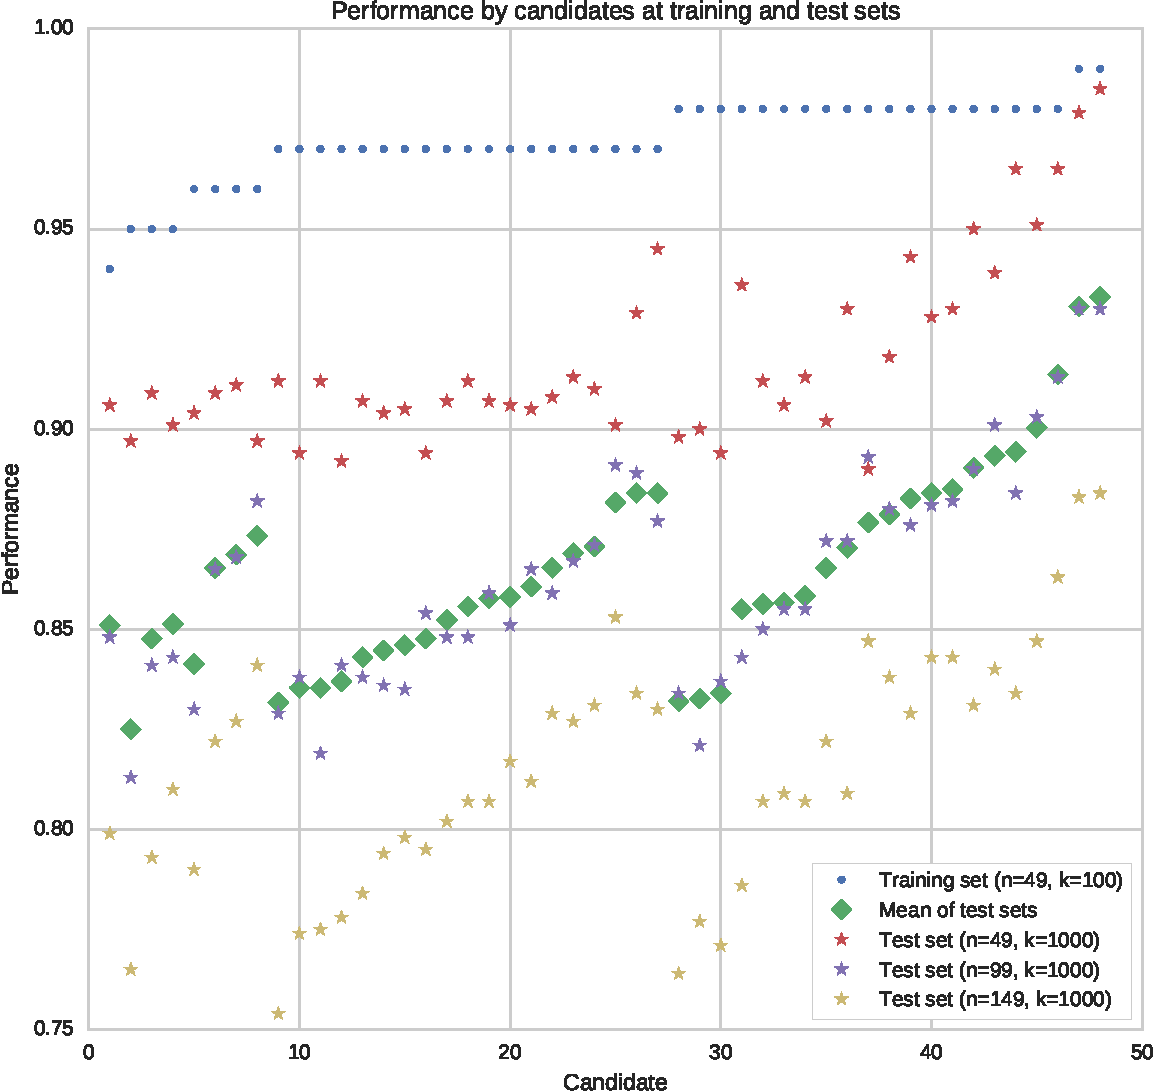
\includegraphics[width=\textwidth, keepaspectratio]{fig/sync_scores}
\caption[
    Performance of the 48 candidate solutions at the training and test sets.
]{
    Performance of the 48 candidate solutions at the training and test sets.
    The candidates have been ordered by training performance first, and average test performance second.
    }
\label{fig:sync_scores}
\end{figure}

Figure \ref{fig:sync_scores} shows the performance of the 48 candidates at the training set and each of the test sets.
It is clear that the candidates that have been trained on $n=49$
There is a correlation between the average score of the test sets and $n$, with the $n=49$ test performing closest to the $n=49$ training performance.
It is also clear that the two candidates that performed the best ($f=0.99$) at the training set, also perform the best at each of the test sets.


%\section{Firing Squad Synchronization Problem}
The \textit{firing squad synchronization problem} is an advanced task for multi-state 1D CA.
From a "resting" starting state the CA must be able to transmit signals so that at some point, every cell simultaneously enters the special "firing" state.

TODO

\section{Investigation of Genome Properties}
\label{sec:properties}
The process of running a task-solving experiments such as in the preceding sections is quite opaque.
The experiment is configured by human, but after it is started the system runs itself with no human input,
and the human observer can only wait and hope a useful result emerges at the end.

In order to gain a better understanding of the process,
an experiment was designed with the goal of investigating various properties of the population and their development over time,
rather than to solve a specific task.
This involves storing every single individual from the whole run, then analyzing them quantitatively afterwards.

CA-NEAT can be studied from multiple "angles": as a GA experiment there are properties such as fitness that can be studied,
as a CA experiment there is for example the $\lambda$ parameterization,
and as a graph-based encoding properties such as the number of nodes can be investigated.
Inspecting these, individually and trying to see correlation, should help with understand the system better,
and selecting better configurations for future experiments.

There are also multiple different mechanisms of the algorithm that can enabled or disabled by configuration.
Running multiple GA runs with different combinations of mechanisms enabled should give some indication about the effects of the mechanism.

\subsection{Experiment Design}
The "Swiss" morphogenesis task is used as the basis for this experiment,
since previous experiments with this problem showed it to be consistently solvable by CA-NEAT, but not trivially simple.
The fitness evaluation for morphogenesis problems is also very fast compared to other problems, making it possible to run tests with large populations in a reasonable amount of time.
The CA for this problem has $K=2$ cell states and the neighborhood shape "Von Neumann" ($N=5$) was used.
An initial population of size $P=1000$ was created, with $N$ input nodes, $K$ output nodes and no initial hidden nodes.
This same population was then used as the initial population for five independent "scenarios" of $G=100$ generations, with different mechanisms of NEAT in use.
Table \ref{tbl:NEAT_incremental} shows which mechanisms are in use in which scenario.
From top to bottom, the table can be read as gradually enabling mechanisms, until arriving at the full algorithm, as used in other experiments.

\begin{table}
    \centering
    \caption{Mechanisms enabled in different scenarios}
    \begin{tabular}{c|ccccc}
    Scenario & Mutation & Crossover & Selection pressure & Speciation & Elitism \\ \hline
    A   & \checkmark        & ~         & ~                  & ~          & ~       \\
    B   & \checkmark        & \checkmark         & ~                  & ~          & ~       \\
    C   & \checkmark        & \checkmark         & \checkmark                  & ~          & ~       \\
    D   & \checkmark        & \checkmark         & \checkmark                  & \checkmark          & ~       \\
    E   & \checkmark        & \checkmark         & \checkmark                  & \checkmark          & \checkmark       \\
    \end{tabular}
    \label{tbl:NEAT_incremental}
\end{table}

\begin{description}
\item[Scenario A] ~\\
Scenario A is different from the rest, since it is not a GA run, but more of a random walk in the search space using the mutation mechanism from the GA.
The individuals present in the initial population are mutated once per generation,
and the mutated versions are recorded as the next "generation".
With no crossover and no selection pressure, the individuals will be completely independent from each other throughout the entire run.
\item[Scenario B] ~\\
Scenario B uses NEAT, however the selection mechanism is completely randomized, so there is no selection pressure towards the goal of accomplishing the morphogenesis task.
\item[Scenario C] ~\\
Scenario C has selection pressure appropriate for the morphogenesis task, but does not use the speciation mechanism of NEAT.
\item[Scenario D] ~\\
Scenario D uses NEAT with selection pressure like C does, but also uses the speciation mechanism.
\item[Scenario E] ~\\
Scenario E uses all mechanisms of NEAT, including a per-species elitism degree of $E=1$.
\end{description}

Unlike the problem-solving experiments, this experiment does not involve multiple trials of the same configurations.
The reasoning is that this would mean we would be studying averages of averages in the following figures,
and some relationships between properties could be hidden by this.
We therefore should not draw any strong conclusions from the observations, but use it to find hypotheses that can be more rigorously investigated later.

\subsection{Fitness}
\begin{figure}
\centering
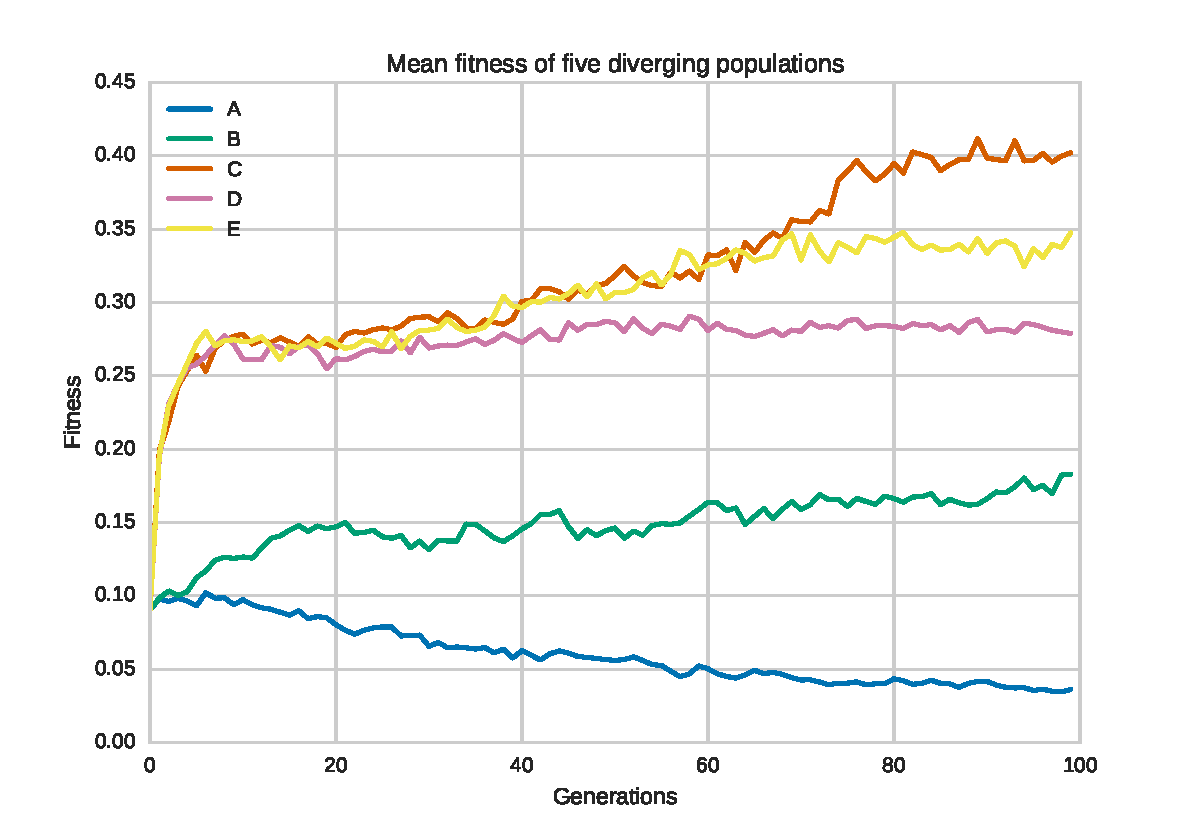
\includegraphics[width=\columnwidth]{fig/fitnesses}
\caption{The development over time of the mean fitness of the populations}
\label{fig:f_over_t}
\end{figure}

\begin{figure}
\centering
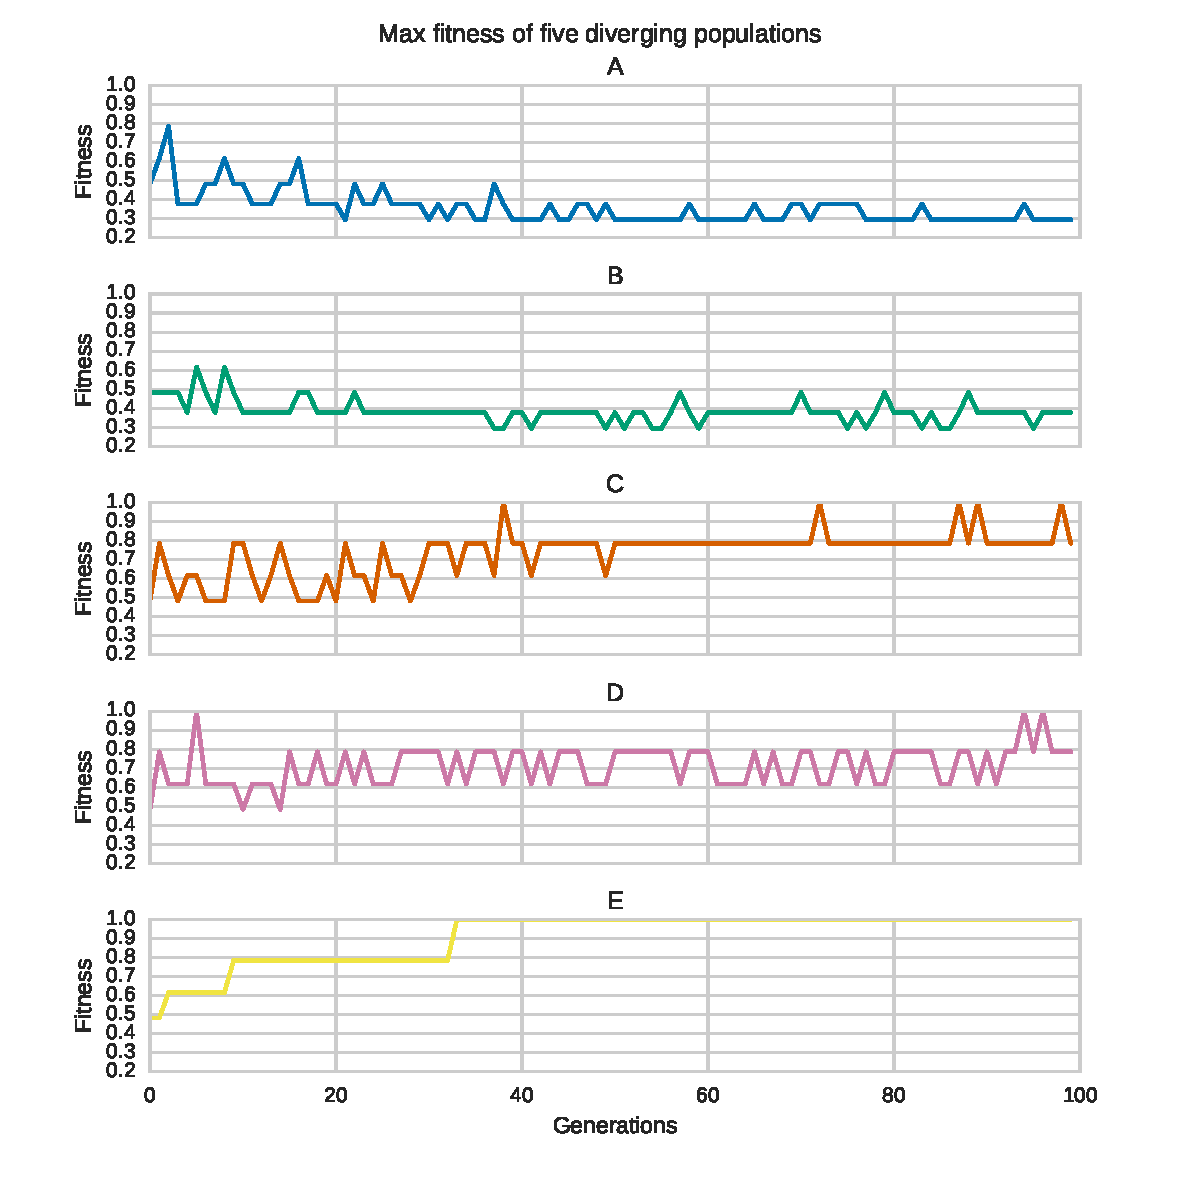
\includegraphics[width=\columnwidth]{fig/fitness_max}
\caption{The development over time of the max fitness of the populations}
\label{fig:max_fitness}
\end{figure}

When working with genetic algorithms, the most obvious property of a population to study is perhaps the average fitness over time.
Figure \ref{fig:f_over_t} shows the mean fitness development across the whole population for each of the five scenarios.
As one would expect, scenario A and B do not show any considerable improvement over time.
A declines steadily, while B has a slight, but not very significant increase.
Among C, D and E, which have selection pressure, there is a sharp increase in the first 10 generations.
D then flattens out for the remaining time, while C and E improves some more, at a slower rate.

Averaging hides one important aspect of the fitness distribution, namely the maximum value, which indicates "success" when it reaches $1.0$.
Looking at the maximum fitness development over time in Figure \ref{fig:max_fitness},
both A and B appears to decline over time, but B less so than A.
C and D act similar in that they hover around the upper half of the scale, sometimes finding a $1.0$ score, but are unable to stay stable there.
Whereas E, with the elitism mechanism is able to stay at $1.0$ once it finds it.
D finds a perfect solution quite early, but this seems likely to be a "fluke", since it losses it again and takes a long time to find another.
This is consistent with the results of the Swiss morphogenesis in Section \ref{sec:prev_work}, where in 100 independent trials, a few of them chanced upon an early solution.

The fact that the C average fitness overtakes both the D and E averages can hypothetically be explained by the difference the speciation mechanism makes.
In scenario C, the search can only optimize for fitness, so when it finds a good candidate it will make a large number of children for that candidate.
Scenarios D and E can optimize for diversity as well, searching in multiple directions.
When a good candidate is found in a species, its children will dominate only in that species,
while the other species continue their search unaffected.
Another possible factor is the stagnation check which is also part of the speciation mechanism.
This eliminates species that haven't improved average fitness in 15 generations.
If a species has "peaked", then it will be eliminated eventually, even if it's average fitness is above the population average.
In the task-solving experiments, the algorithm is stopped when a "perfect" solution is found, but in this experiment it is allowed to continue, so this effect can happen.

\subsection{Speciation}
\begin{figure}
\centering
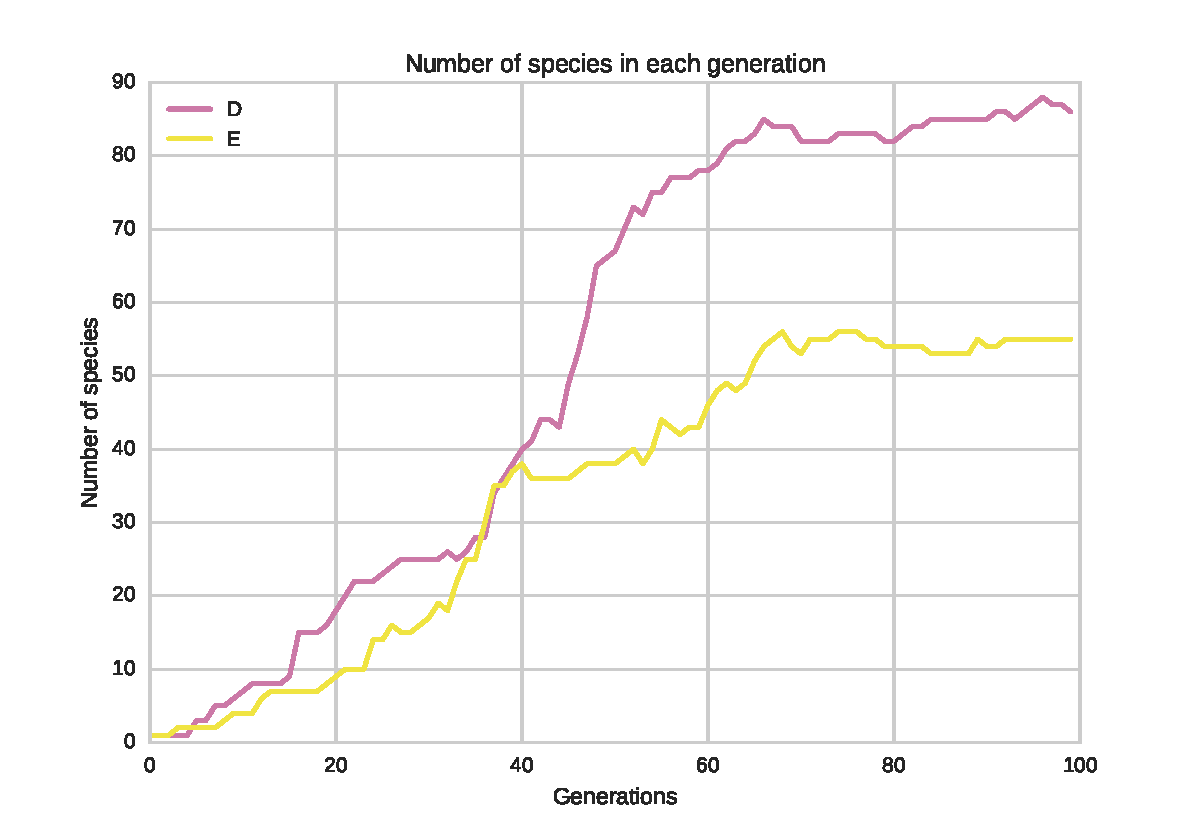
\includegraphics[width=\columnwidth]{fig/species}
\caption{The number of species in scenarios D and E over time}
\label{fig:species}
\end{figure}

\begin{figure}
\centering
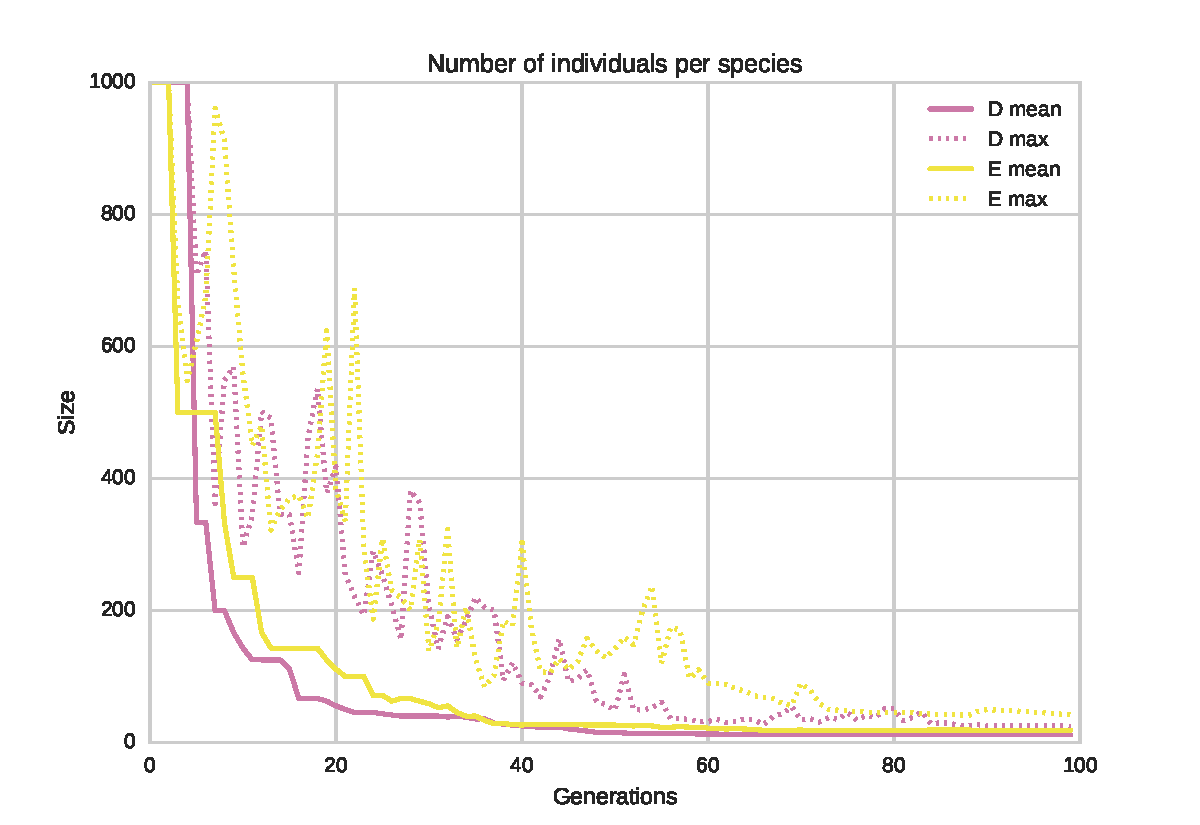
\includegraphics[width=\columnwidth]{fig/species_size}
\caption{The mean and max number of members in the species of scenarios D and E over time}
\label{fig:species_size}
\end{figure}

Another GA property that can be studied is the NEAT-specific speciation in scenarios D and E.
Figure \ref{fig:species} shows the number of different species over time.
Both follow approximately the same development in the first 40 generations, before D overtakes E and they stabilize at different levels.
The difference in levels is quite significant.
A speculative reason for this is that the lack of elitism in D means that a species there is more likely to split into multiple species by chance.
Whereas with elitism in E, the members of the species may be more likely to remain more similar to the elite in the population, leading to less diversity \textit{within} the species.

Figure \ref{fig:species_size} shows the mean number of members per species over time.
The development is as one would expect with the growing number of species seen in Figure \ref{fig:species}, declining more rapidly at first then gradually stabilizing.
The accompanying plot of the max number of species members gives an indication of the variance of the underlying data.
It fluctuates a lot at first, but as 100 generations approach,
the max stabilizes and is only slightly higher than the mean, indicating that the population consists of many species approximately the same (low) number of members.

In the case where there is elitism, as the species size approaches the number of elites ($E=1$) there is less room for innovation in that species, since one member of each species is always a copy of a previous one.
If the size were to reach $1$, there would be no innovation at all happening.
Since the population of scenario E seems to have stabilized around 55 species, a mean species size around $1000 / 55 \approx 18$ should avoid this problem and leave room for innovation.

\subsection{$\lambda$}
\begin{figure}
\centering
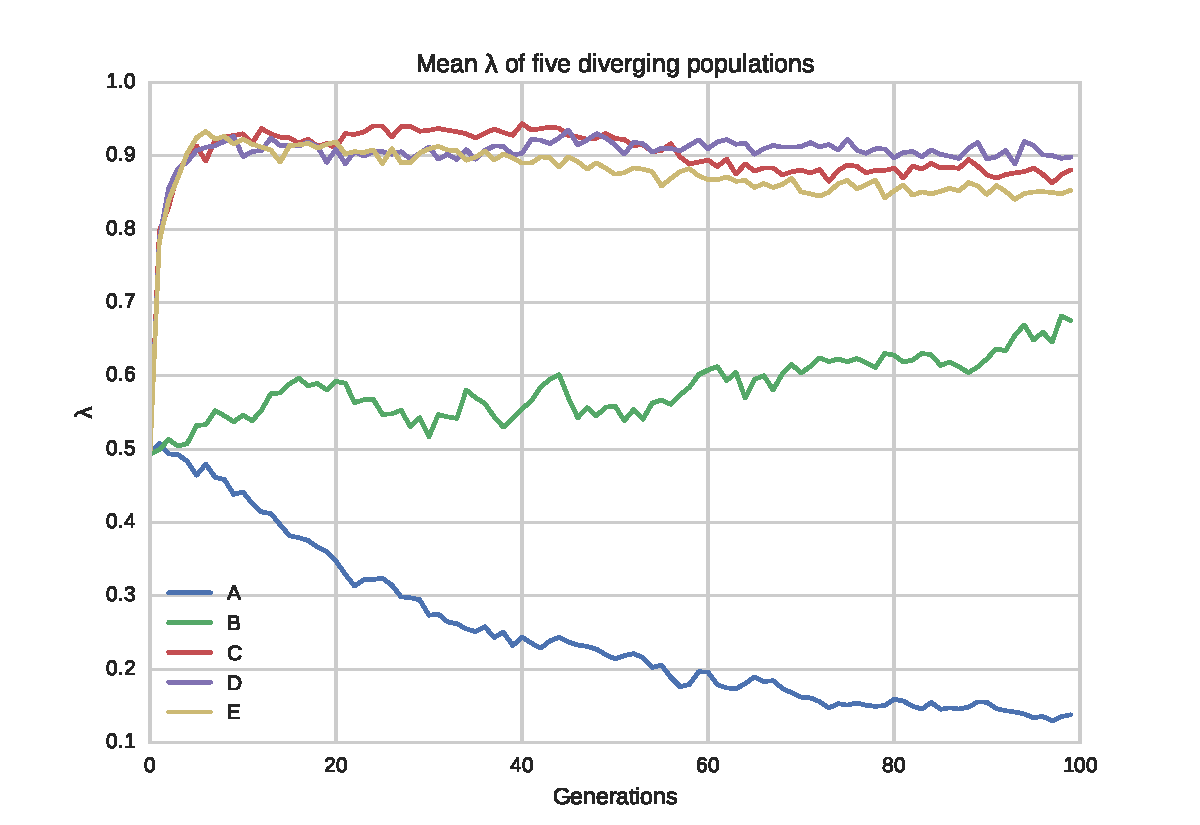
\includegraphics[width=\columnwidth]{fig/mean_lambda}
\caption{Development of the mean $\lambda$ of five scenarios over time}
\label{fig:lambda_over_t}
\end{figure}

\begin{figure}
\centering
\begin{subfigure}[t]{.49\columnwidth}
\centering
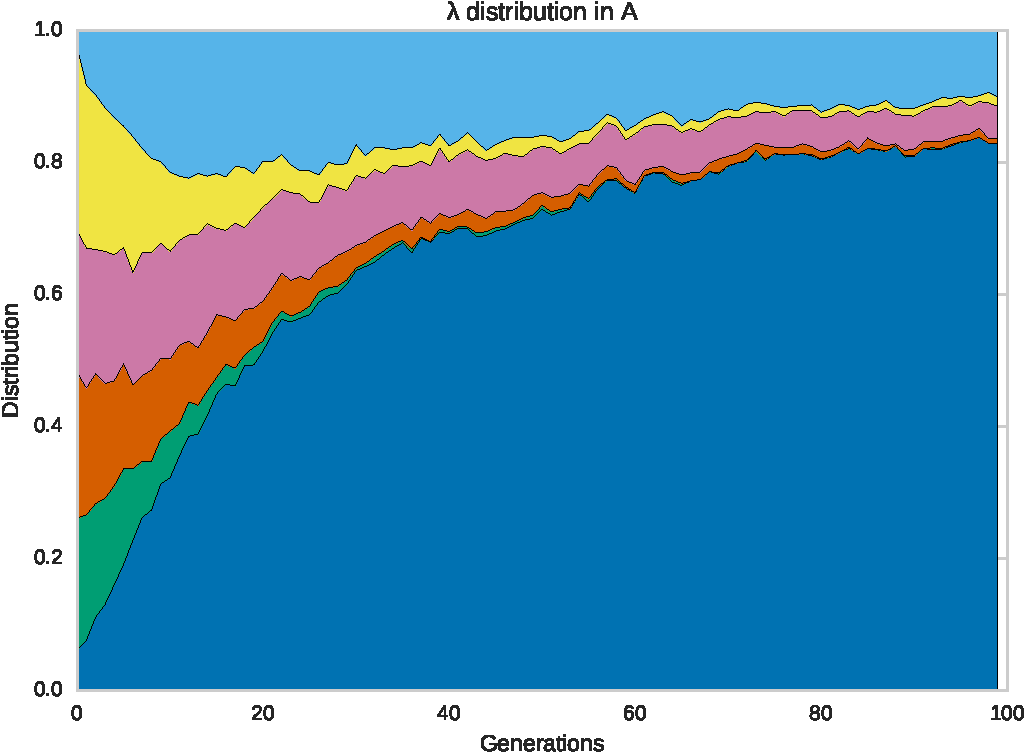
\includegraphics[width=\columnwidth]{fig/lambda_A}
\caption{Scenario A}
\label{fig:lambda_A}
\end{subfigure}
\begin{subfigure}[t]{.49\columnwidth}
\centering
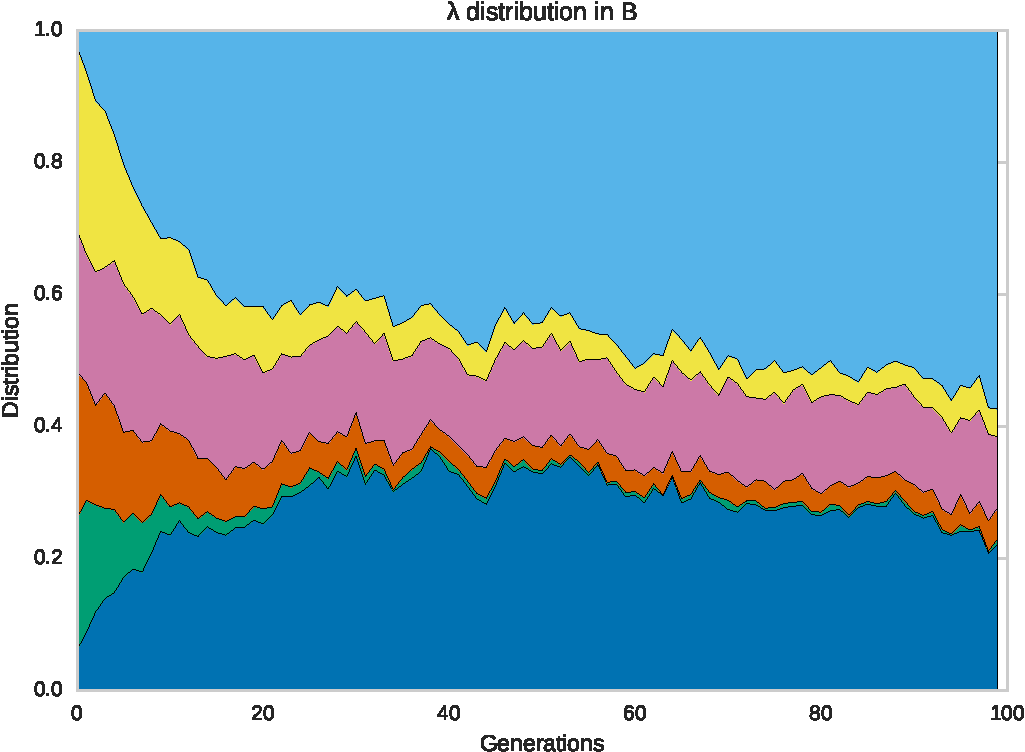
\includegraphics[width=\columnwidth]{fig/lambda_B}
\caption{Scenario B}
\label{fig:lambda_B}
\end{subfigure}
\begin{subfigure}[t]{.49\columnwidth}
\centering
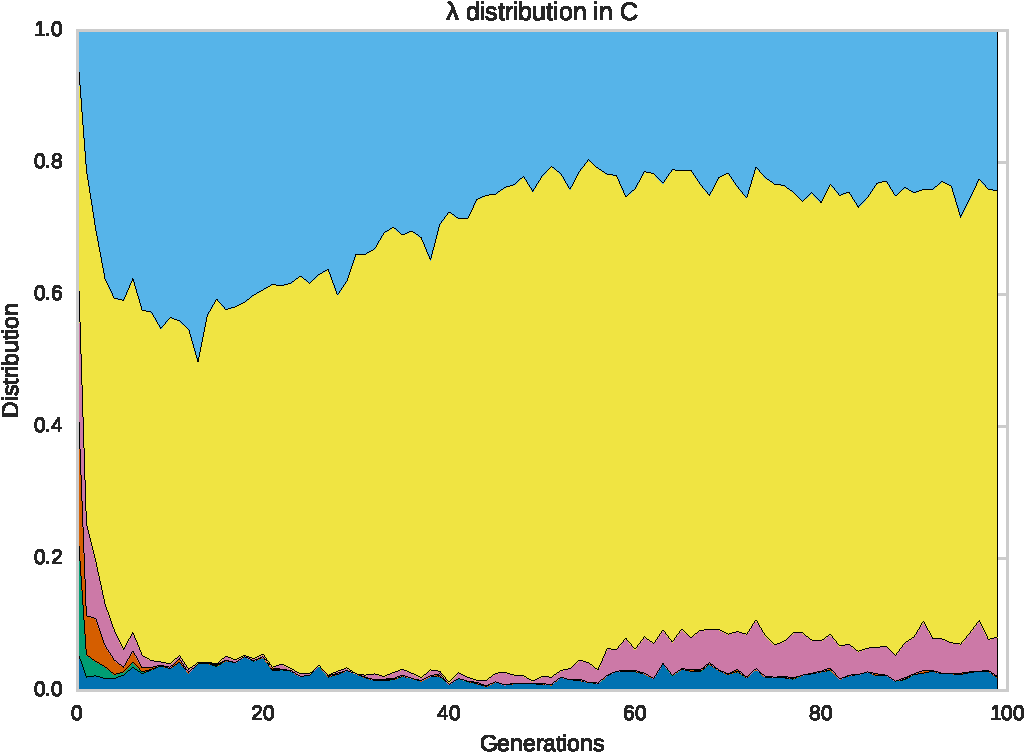
\includegraphics[width=\columnwidth]{fig/lambda_C}
\caption{Scenario C}
\label{fig:lambda_C}
\end{subfigure}
\begin{subfigure}[t]{.49\columnwidth}
\centering
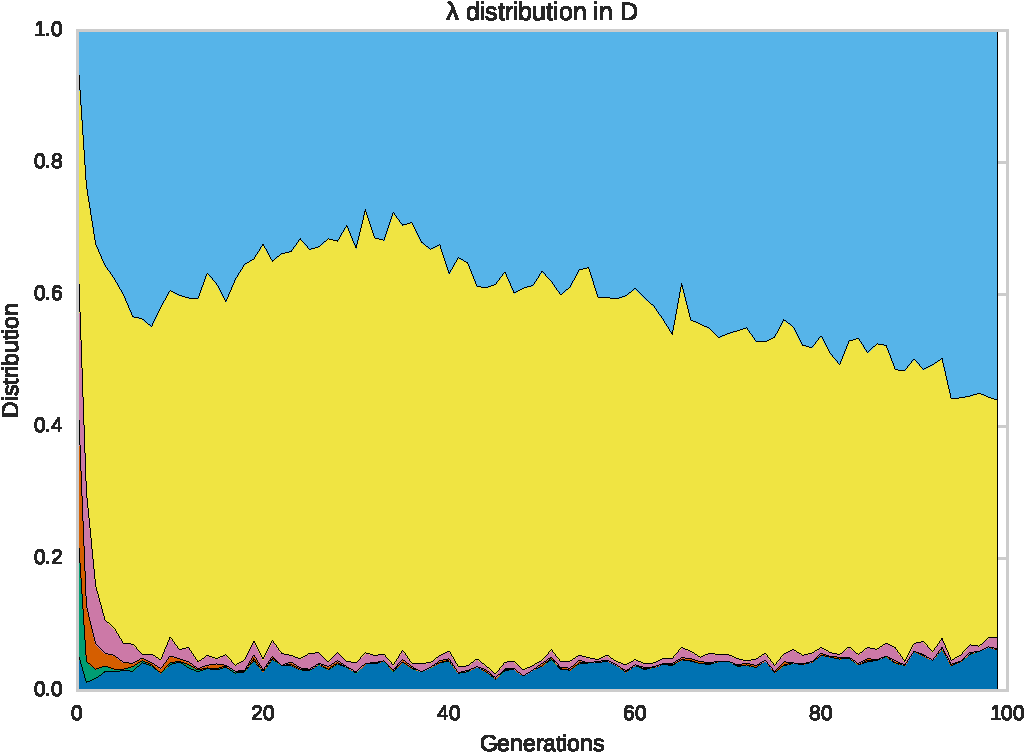
\includegraphics[width=\columnwidth]{fig/lambda_D}
\caption{Scenario D}
\label{fig:lambda_D}
\end{subfigure}
\begin{subfigure}[t]{.49\columnwidth}
\centering
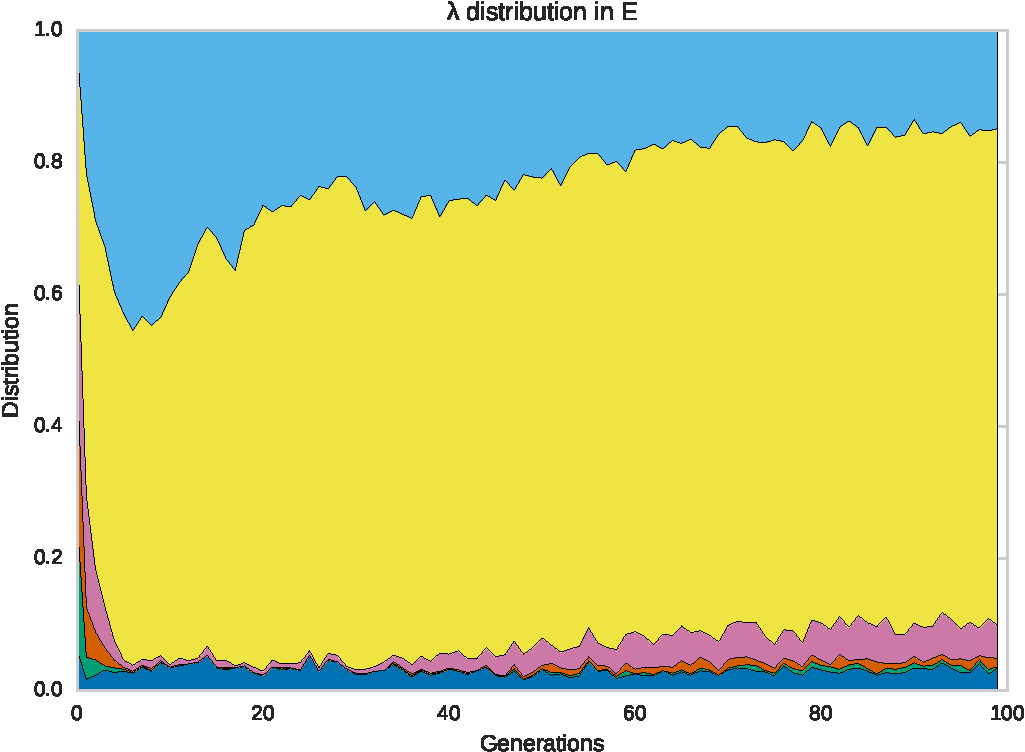
\includegraphics[width=\columnwidth]{fig/lambda_E}
\caption{Scenario E}
\label{fig:lambda_E}
\end{subfigure}
\begin{subfigure}[t]{.49\columnwidth}
\centering
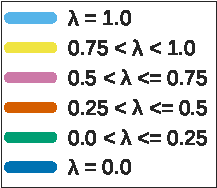
\includegraphics[width=\columnwidth, height=4.5cm, keepaspectratio]{fig/lambda_legend}
\caption{Legend}
\end{subfigure}

\caption{Breakdown of $\lambda$ distribution over time in five scenarios}
\label{fig:lambdas_breakdown}
\end{figure}

The $\lambda$ parameter is an interesting property of a CA transition function to study.
Figure \ref{fig:lambda_over_t} shows the mean $\lambda$ over time for the five scenarios.
The shapes of the curves have a lot of similarities with the shapes of the fitness curves in Figure \ref{fig:f_over_t}.
The random mutation in scenario A drives the mean $\lambda$ towards $0$,
while the combination of mutation and crossover without selection pressure of scenario B causes the $\lambda$ to fluctuate a lot and increase slightly, but not very significantly.
Scenarios C, D and E have roughly the same development: a sharp rise to about $0.9$, then flattening out.
%Both D and E do a slight "correction" afterwards, slowly decreasing after the initial rapid rise.

Figure \ref{fig:lambdas_breakdown} shows the scenarios broken down individually into stack plots, illustrating the distribution of values changing over time.
The values are sorted into six bins, two special ones for $\lambda$ exactly equal to $0.0$ and $1.0$ and four for the equal intervals in between.
In earlier experiments it was observed that the two extreme $\lambda$ occur often, so they get special bins in this visualization.

It can be seen that the scenario A has a very strong bias towards producing $\lambda = 0.0$,
while the other scenarios skew more towards producing higher $\lambda$ values.
This would suggest that crossover mechanism is at least partially responsible for producing higher $\lambda$ values.
There is also a strong resemblance between C and E, less so between D and the others.
Why this is so is not entirely obvious, but it could just be a consequence of the randomness of the trial.
If the experiment was repeated with multiple trials, we could determine if this is just a fluke or not.
In any case, it is clear that all the scenarios with selection pressure are strongly biased towards producing $\lambda > 0.75$.

The task at hand and the implementation of the fitness function must also be considered when analyzing the $\lambda$ result.
The fitness evaluation function is described in detail in Section \ref{sec:morph_problems}.
Notably, when trying to produce a "Swiss flag" pattern, 
$20/25$ cells are active in the target state, meaning that the algorithm can get \textit{some} score easily by producing a transition function with $\lambda = 1.0$.
This can explain why the algorithm produces very many $\lambda=1.0$ solutions early on.
%Considering this, as well as Langton's theory of the "Edge of Chaos", the breakdowns seen in C, D and E make sense.

%\begin{figure}
%\centering
%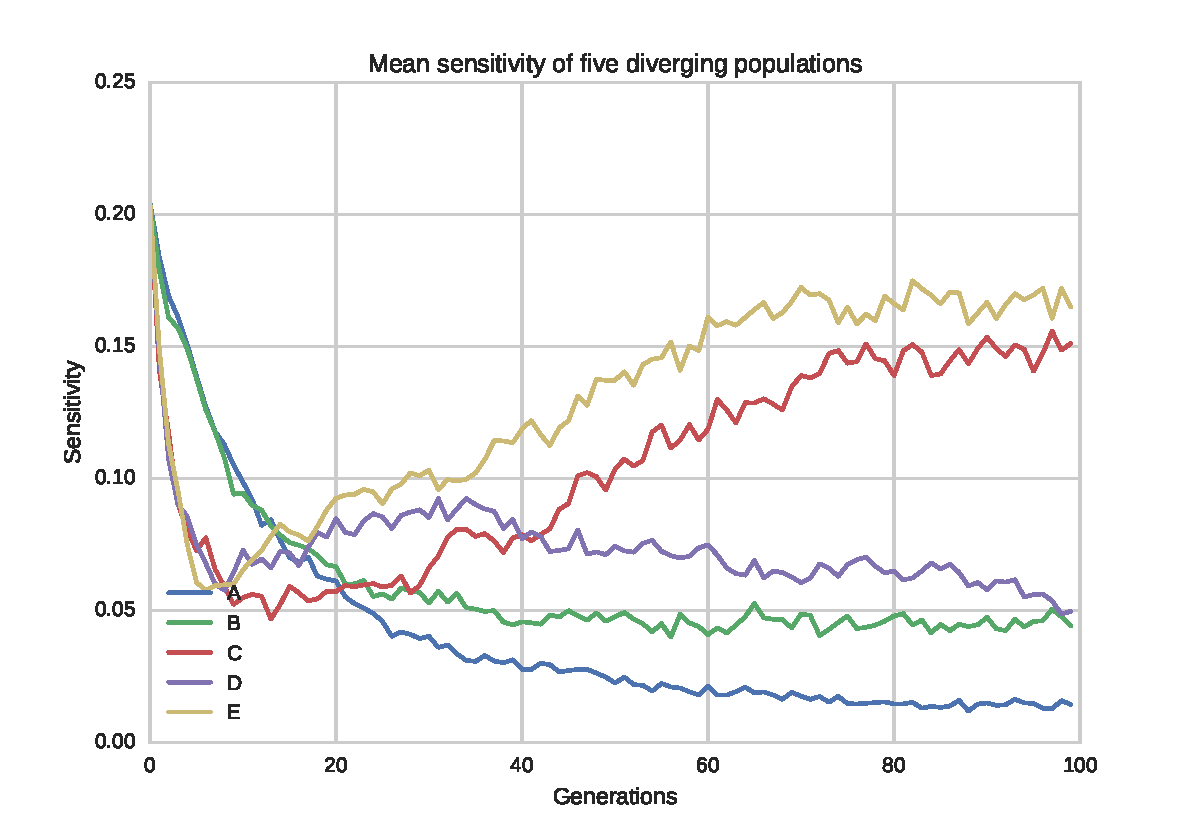
\includegraphics[width=\columnwidth]{fig/sensitivity}
%\caption{TODO}
%\label{fig:sensitivity}
%\end{figure}

%\begin{figure}
%\centering
%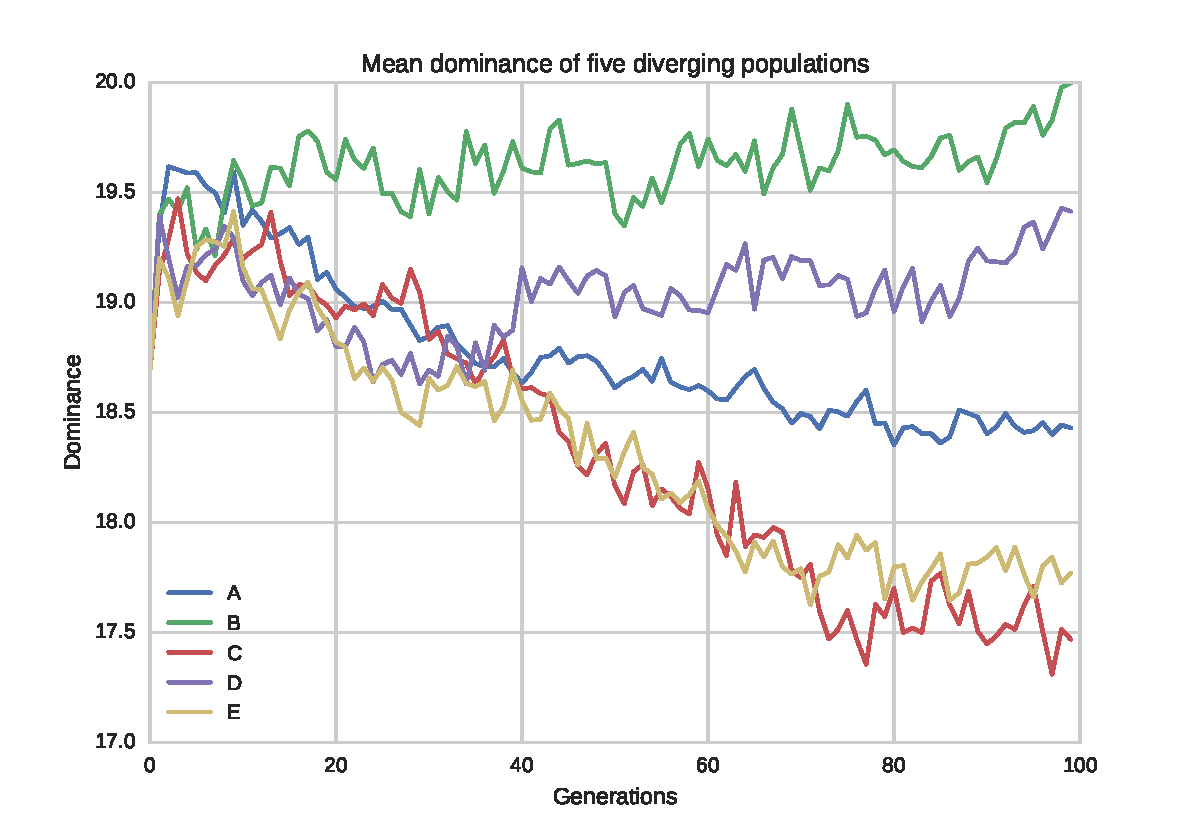
\includegraphics[width=\columnwidth]{fig/dominance}
%\caption{TODO}
%\label{fig:dominance}
%\end{figure}


\subsection{Distinct behaviors}
\begin{figure}
\centering
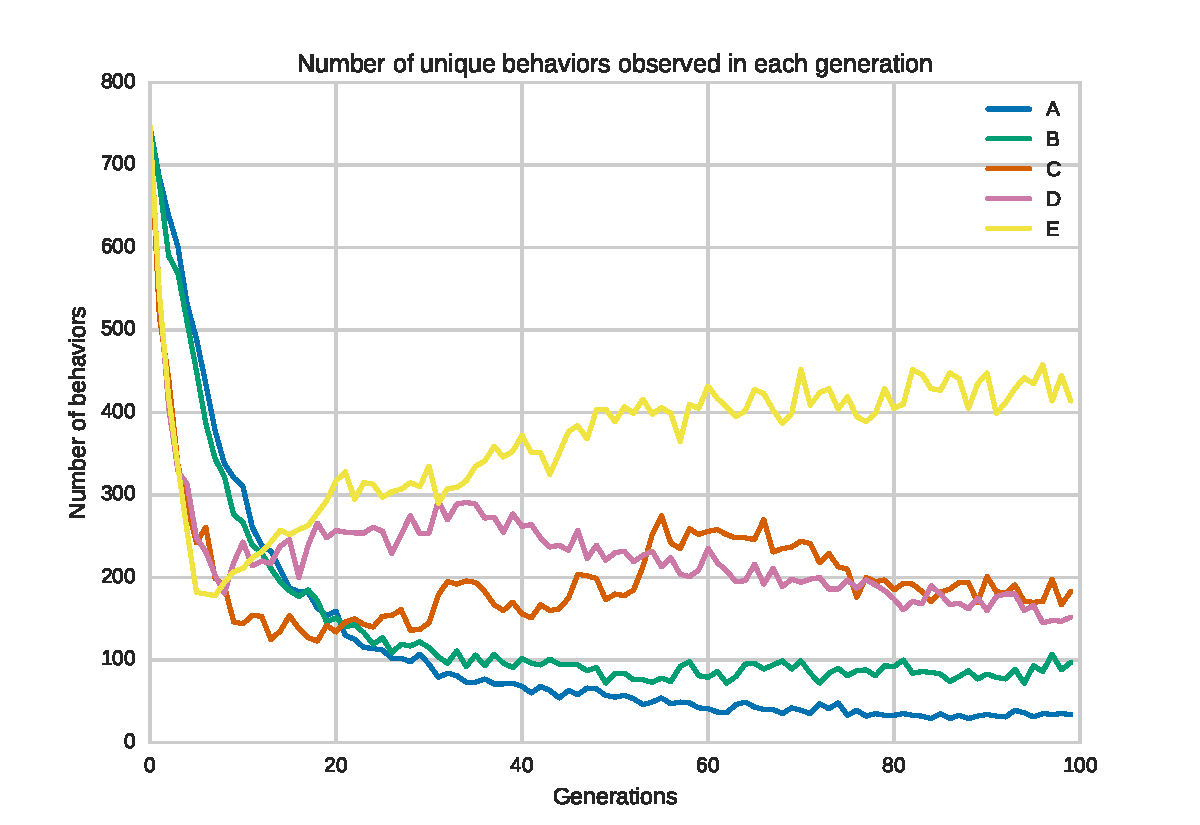
\includegraphics[width=\columnwidth]{fig/unique_behaviors}
\caption{Number of unique behaviors in each generation}
\label{fig:unique_behaviors}
\end{figure}

\begin{figure}
\centering
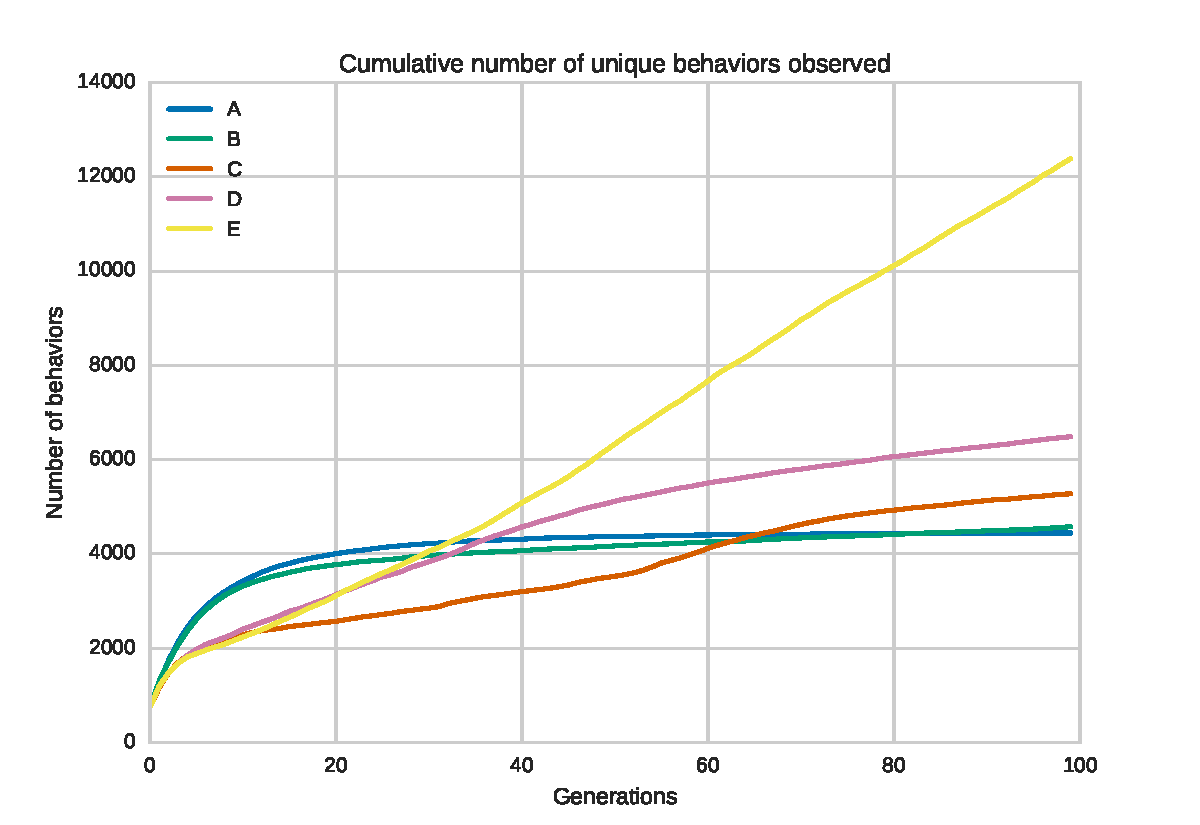
\includegraphics[width=\columnwidth]{fig/cummulative_unique_behaviors}
\caption{
    Number of unique behaviors seen over time, cumulative.
}
\label{fig:cummulative_unique_behaviors}
\end{figure}

\begin{figure}
\centering
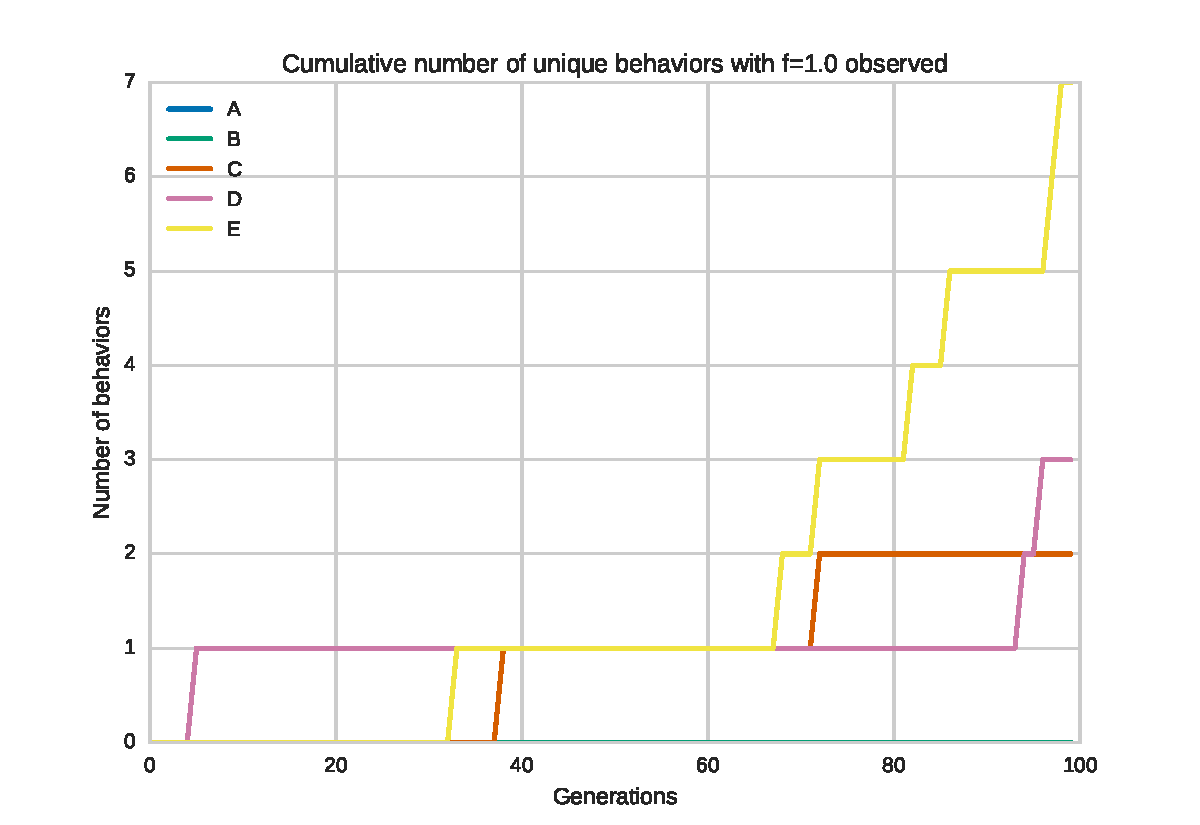
\includegraphics[width=\columnwidth]{fig/cummulative_unique_perfect}
\caption{
    Number of unique $f=1.0$ behaviors seen over time, cumulative.
}
\label{fig:cummulative_unique_perfect}
\end{figure}

%\begin{figure}
%\centering
%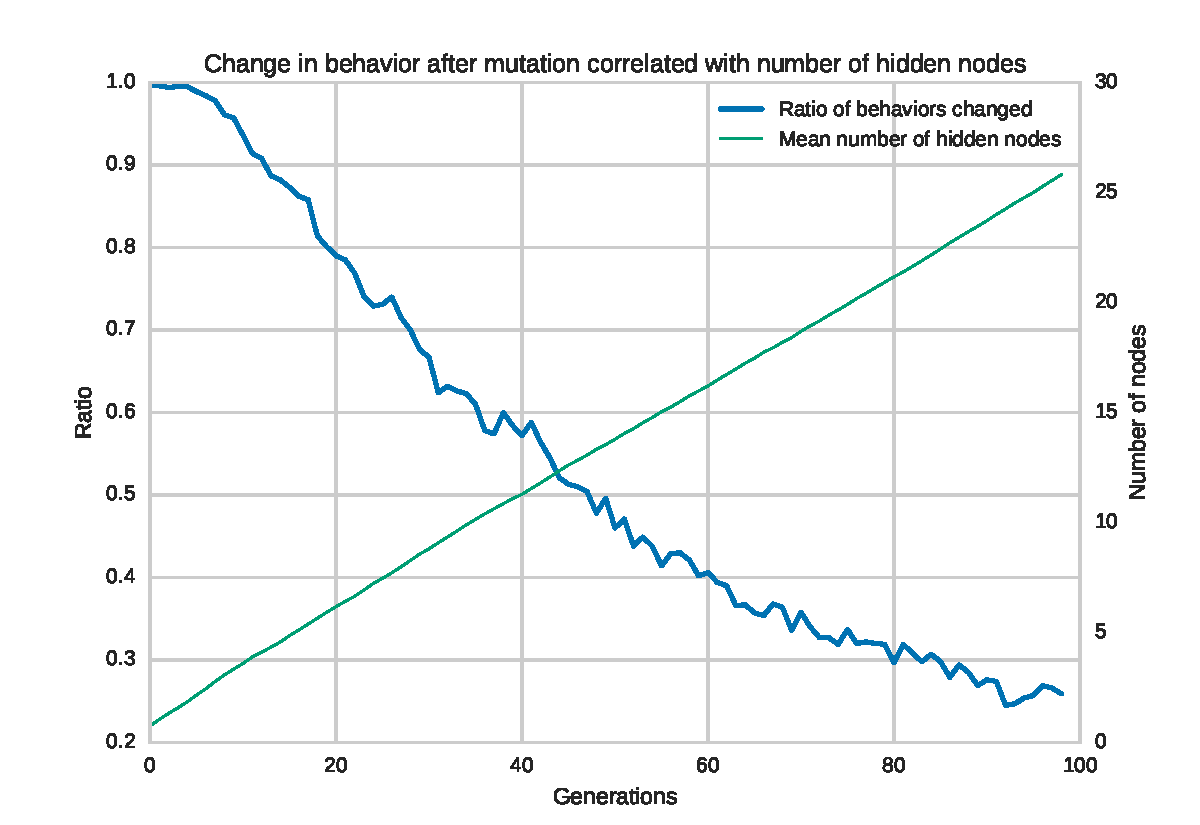
\includegraphics[width=\columnwidth]{fig/mutation_behavior_change}
%\caption{Ratio of genotypes that change behavior after mutation}
%\label{fig:mutation_behavior_change}
%\end{figure}

%Studying the $\lambda$ parameter can give some insights, but it does not capture every aspect of the transition function behavior.
Another way to analyze the population is to look at the diversity of the enumerated behavior "strings" over time.
Figure \ref{fig:unique_behaviors} shows how many unique behaviors are present in each generation of each scenario.
The initial population is clearly very diverse, but the diversity drops very rapidly in each of the scenarios.
Scenarios A and B decrease slightly slower than the rest at the beginning.
The rate of decreasing slows down and they eventually stabilize at low levels.
Scenarios C, D and E drop down fast at first, but then they do a sharp turn.
C and D fluctuate a it up and down, but overall seem to stabilize.
E rises steadily again and stabilizes at a significantly higher level than the others.

Figure \ref{fig:cummulative_unique_behaviors} visualizes the number of unique behaviors seen in the entire lifetime of the scenario.
A and B are almost identical, showing almost no increase after the first 20 generations.
C and D climb steadily and overtake A and B at different points.
The contrast between E and the rest is stark.
There is a much higher rate of increase, and it is almost linear over time, reaching about twice the value that the next best does in 100 generations.
These result have some big implications.
First of all, it is clear that a random search such as A and B gets "stuck" quite quickly and stops producing innovative results.
With selection pressure, the search is slower at first, needing quite some time to overtake the initial flood of innovation produced by randomness.
But it keeps a steady increase where the random search stops.
And the presence of elitism increases the innovation by a very considerable degree.

In a "best-case" where every behavior in every generation is distinct,
the number of unique behaviors observed would be $P * G = 100000$.
Scenario E passes 12000 unique behaviors observed, which is "only" 12\% of the theoretical maximum.
And for a $K=2, N=5$ CA, the number of total possible behaviors is $K^{K^N} = 2^{32} \approx 4.3 * 10^9$.
This illustrates the futility of attempting to solve advanced CA tasks by exhaustive enumeration of behaviors.
Luckily, while the proverbial haystack may be humongous,
there are many needles to be found within it, and you only need to find one to be successful.
Figure \ref{fig:cummulative_unique_perfect} illustrates the number of distinct behaviors observed with a perfect fitness score.
As one might expect, the diversity of the optimal behaviors is higher when the diversity of all behaviors is higher.
Scenario E is able to find 7 distinct solutions to the task.

\subsection{Network Topology}
\begin{figure}
\centering
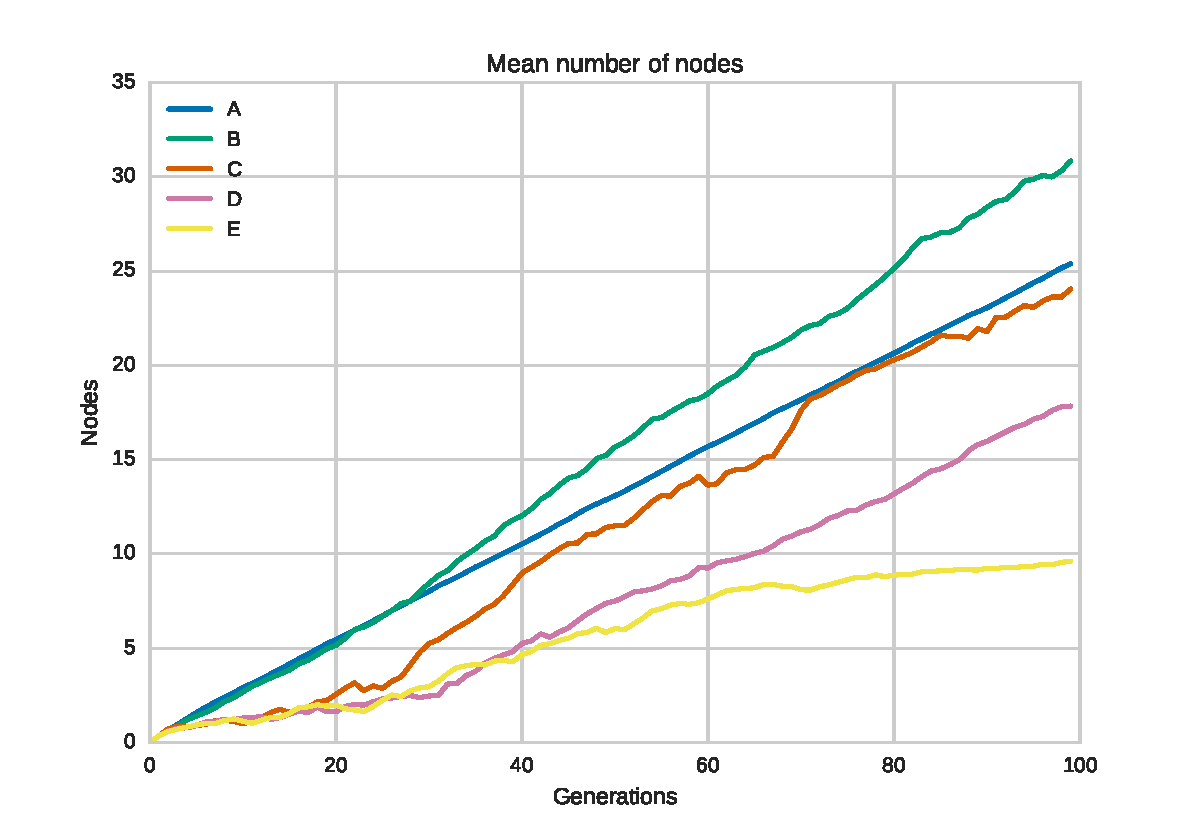
\includegraphics[width=\columnwidth]{fig/sizes}
\caption{The mean number of nodes in each scenario}
\label{fig:sizes}
\end{figure}

\begin{figure}
\centering
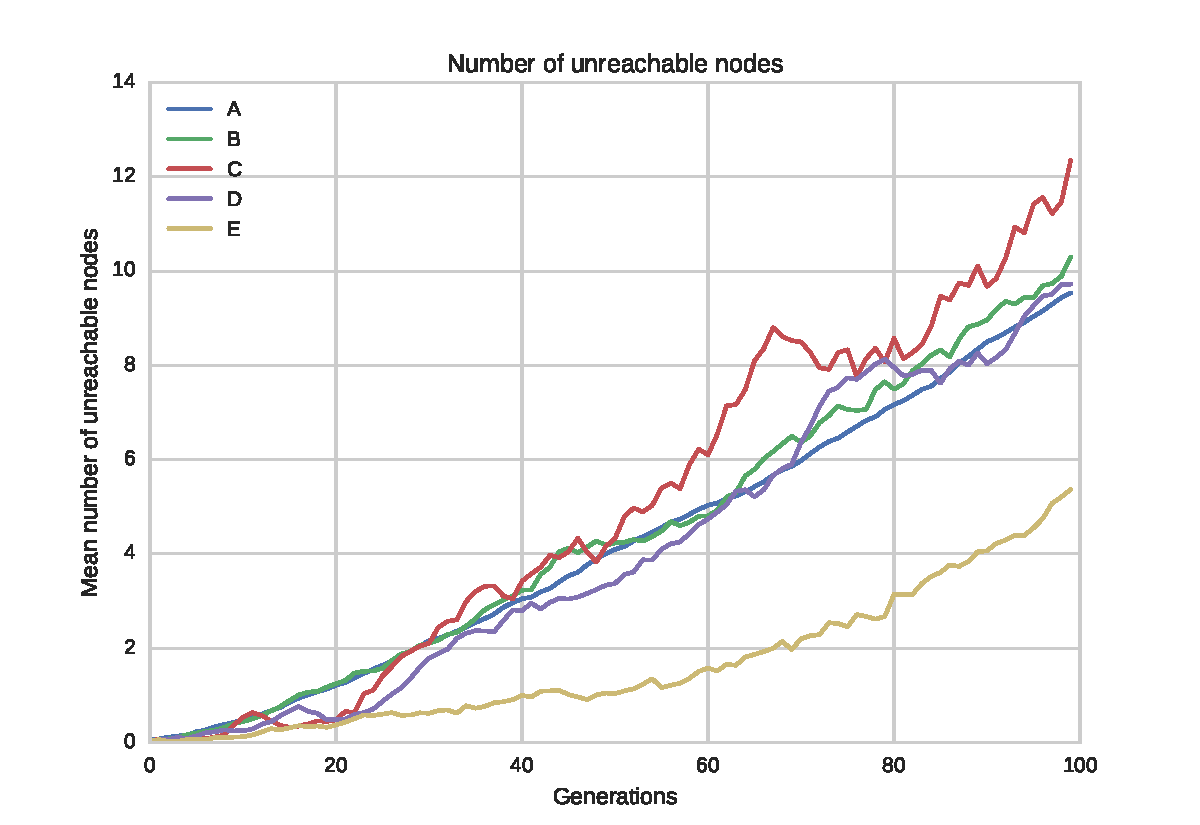
\includegraphics[width=\columnwidth]{fig/vestigial_nodes}
\caption{The mean number of disconnected nodes in each scenario}
\label{fig:vestigial_nodes}
\end{figure}

%\begin{figure}
%\centering
%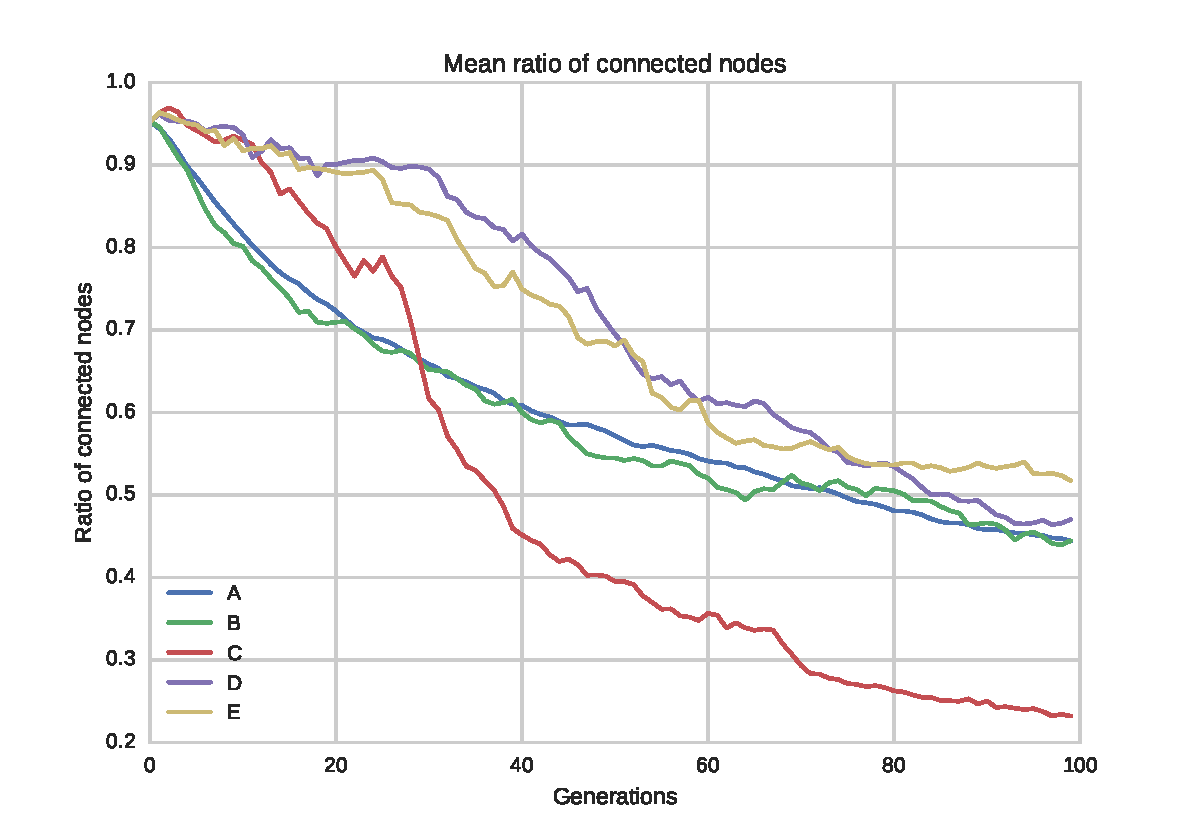
\includegraphics[width=\columnwidth]{fig/vestigial_ratio}
%\caption{The ratio of connected nodes in each scenario}
%\label{fig:vestigial_ratio}
%\end{figure}

\begin{figure}
\centering
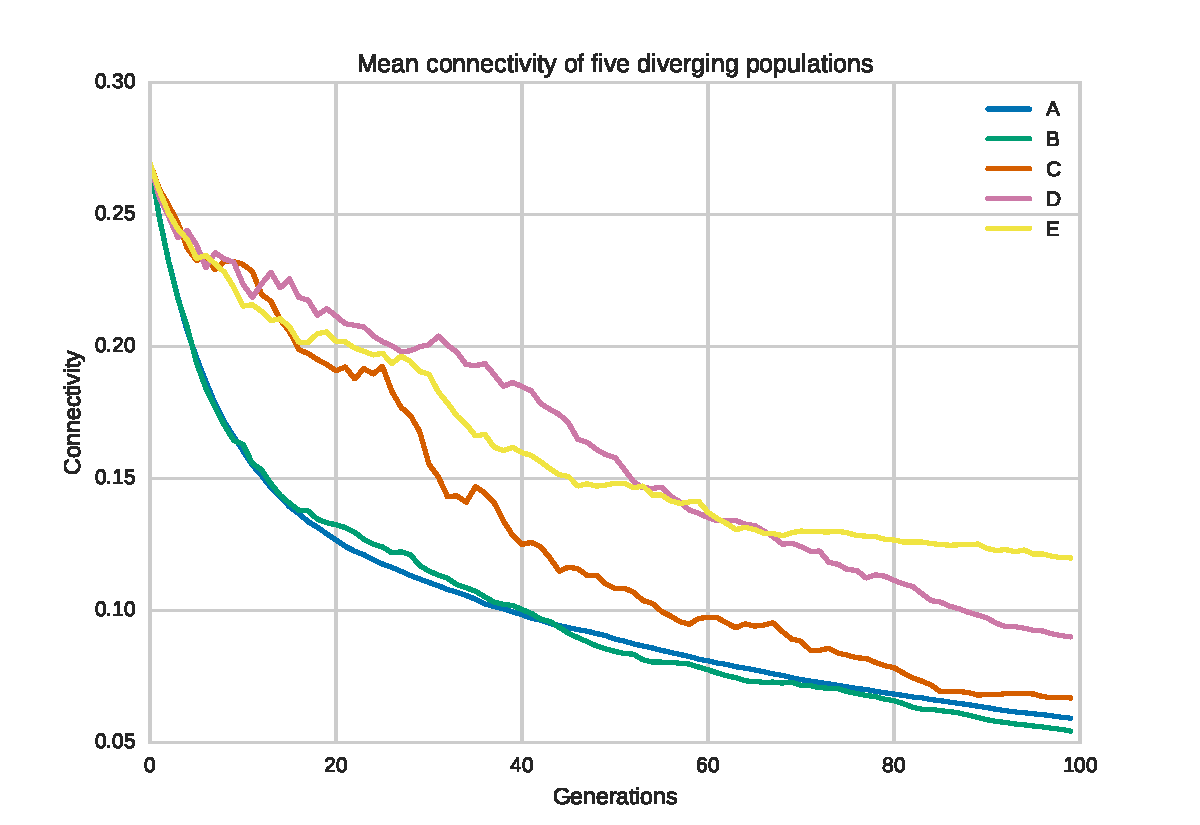
\includegraphics[width=\columnwidth]{fig/connectivity}
\caption{The mean connectivity degree in each population}
\label{fig:connectivity}
\end{figure}

The individuals of the populations are graph structures, and can also be studied as such.
Figure \ref{fig:sizes} shows the development of the mean number of nodes in the networks of each scenario.
The growth of scenario A is approximately linear.
Since the individuals of the population are completely independent from each other,
the law of large numbers means that the curve should fit the expected value given by the probabilities of adding and removing nodes, $(P_\text{add} - P_\text{remove})x = (0.5 - 0.25)x = 0.25x$.
This is not a very useful insight by itself, but it does give a baseline which the other scenarios can be compared to.
Scenario B has a slightly higher growth than A.
This makes sense considering the crossover mechanism.
If two parents independently are likely to gain a new node, then their child will have both of the new nodes, leading to a bigger growth rate overall.
The three scenarios with selection pressure at first follow the same pattern, with much lower growth than the baseline.
Then they diverge around 30 generations.
Scenario C "catches up" with scenario A and settles into a near-linear growth like scenario A.
Scenario D also goes into a linear growth close to the same as scenario A, but without "catching up" first.
Scenario E continues with almost the same growth rate for all 100 generations, ending up at a much lower number than the rest.

Figure \ref{fig:vestigial_nodes} shows the number of "vestigial" nodes that do not connect to the output layer.
The significance of these is that they are equally likely to be affected by mutation as any other node, but they do not affect the output of the network.
The more vestigial nodes there are, the more likely that the mutation operation does "nothing".

Scenarios A and B have curve shapes very similar to those they had in Figure \ref{fig:sizes}, suggesting a simple proportional correlation when the process is completely random.
More interestingly, the curve of scenario C does a sudden turn to overtake both A and B.
The curve of C reaches almost the same value as that in Figure \ref{fig:sizes}, indicating the population members have a very large number of disconnected nodes.
The curves of D and E are similar to their counterparts in Figure \ref{fig:sizes}.
Again it is clear that E has a distinctly different development than the rest.

%Figure \ref{fig:vestigial_ratio} shows the relationship between Figures \ref{fig:sizes} and \ref{fig:vestigial_nodes}.
%Scenarios A and B run a very parallel course here, as does D and E.
%The four actually end up near the same value at 100 generations.
%C on the other hand, goes off to do its own thing completely here, and as noted earlier, ends up at a very low ratio of connectedness.

Figure \ref{fig:connectivity} shows another measure of connectedness which is often used in graph theory, $\text{connectivity} = \frac{c}{\sum_{x=1}^{n}{x}}$, where $c$ is the number of connections and $n$ is the number of nodes.
In this perspective, C follows D and E at first, but diverges and drops much quicker to the level of A and B.

What these observations seem to indicate, is that the population of C comes to be dominated by networks with many nodes and fewer connections.
It is likely that in repeated trial this would not occur every time, but that it is just part of the randomness of the single trial.
This is perhaps more likely to occur with the scenario C parameters than the others.
Scenarios A and B are somewhat predictable systems with behavior determined by the constant parameters set before the experiment.
The selection pressure of C can possibly act as a feedback loop, causing a random feature to dominate the whole population.
Scenarios D and E have speciation which automatically create (somewhat) independent trials within the population.

TODO round off this section with some overarching general discussion, maybe in the next chapter

\section{Novelty Search}
Section \ref{sec:novelty} describes how CA-NEAT was extended to support novelty search.

Because novelty search disregards the objective,
a search for a specific neighborhood size $N$ and number of states $K$ creates population that can be used on any CA with that $N$ or $K$.
For example, the same population could contain solutions to both morphogenesis and replication of both the 6x6 "Tricolor" and 7x7 "Nordic" patterns (Figure \ref{fig:patterns}).

\subsection{Results}
\begin{figure}
\centering
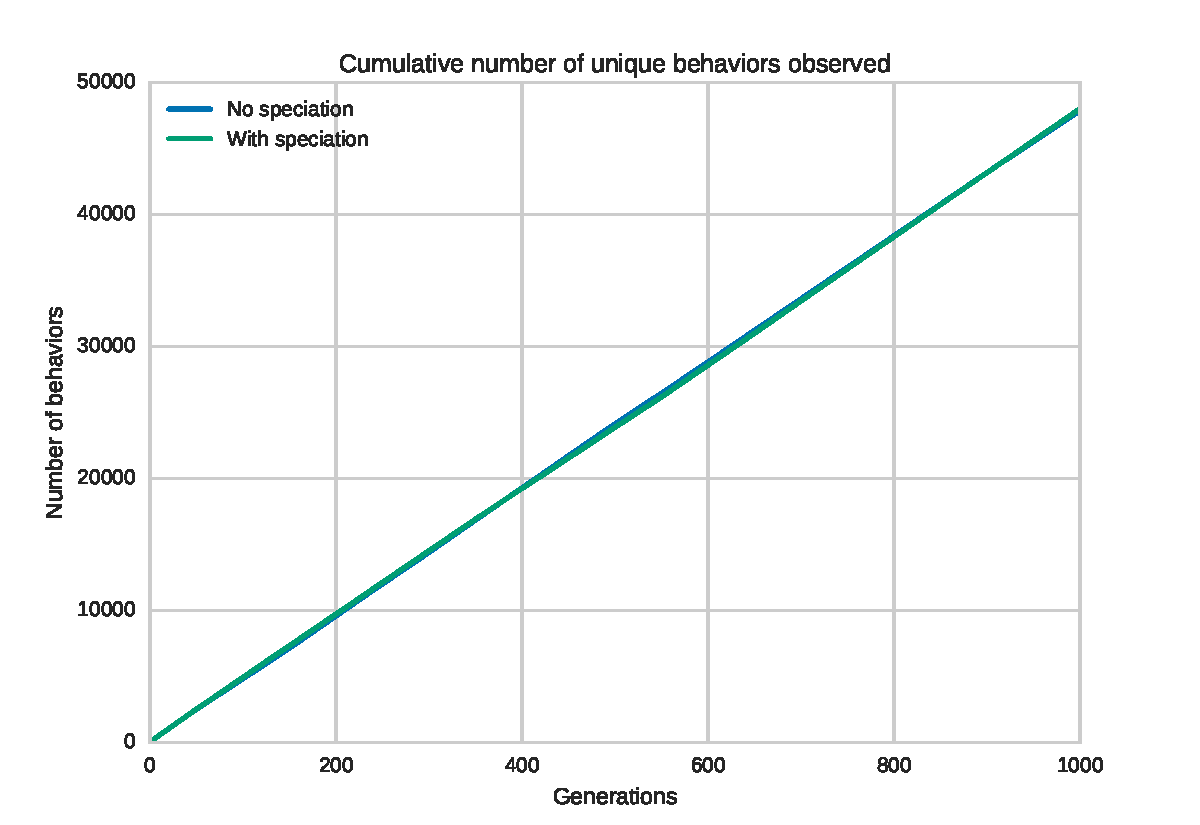
\includegraphics[height=0.4\textheight, width=\textwidth, keepaspectratio]{fig/novelty_diversity}
\caption[
    Cumulative number of unique behaviors observed
]{
    Cumulative number of unique behaviors observed.
    The two runs share the properties $N=5, K=4, P=50, G=1000$, and differ in whether they have speciation enabled.
}
\label{fig:novelty_diversity}
\end{figure}

\begin{figure}
\centering
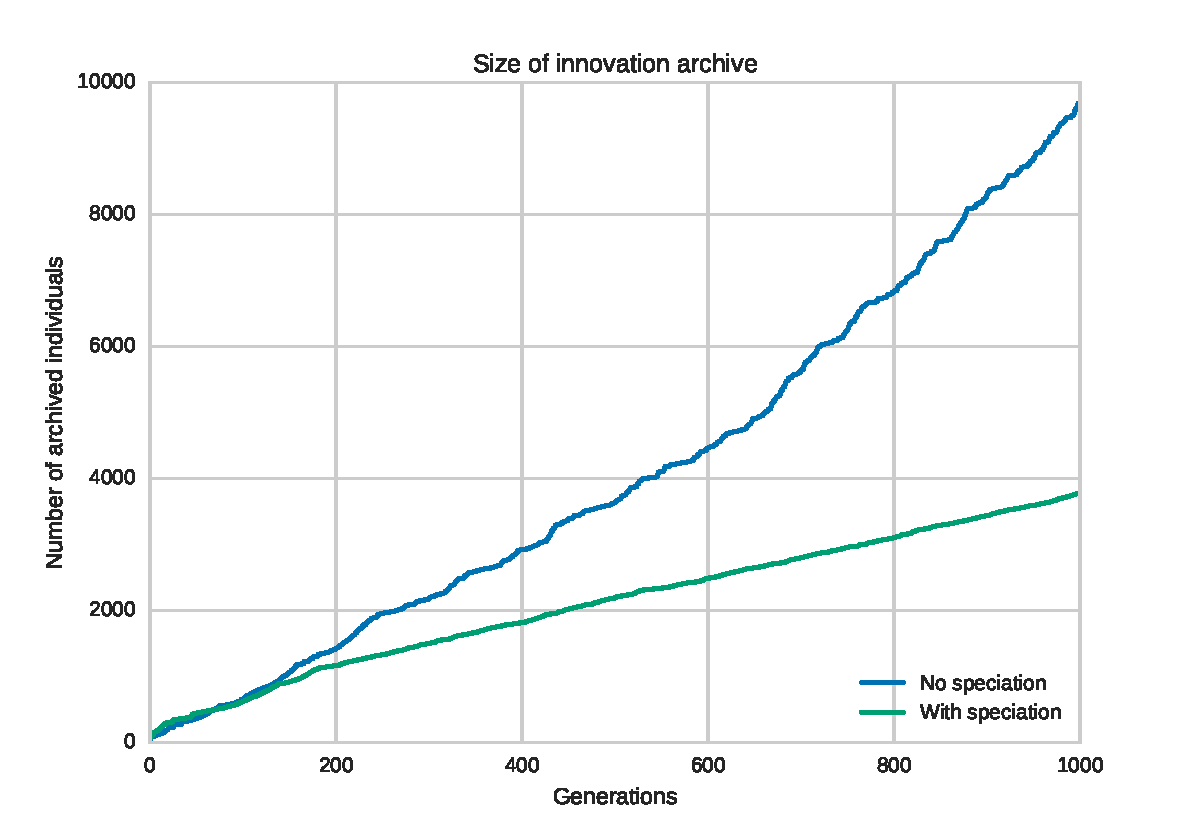
\includegraphics[height=0.4\textheight, width=\textwidth, keepaspectratio]{fig/innovation_archive_size}
\caption[
    Size of the innovation archives
]{
    Size of the innovation archives.
    The archives are a subset of their corresponding populations.
}
\label{fig:innovation_archive_size}
\end{figure}

\begin{table}
\centering
\caption{Overview of the novelty search runs attempted}
\begin{tabular}{c|c|c|c|c|l}
    N   &   K   &   P   &   G   &   Speciation  &   Objectives tested   \\\hline
    5   &   4   &   50  &   1000    &   Yes &   \{Swiss, Nordic\} \{morphogenesis, replication\} \\
    5   &   4   &   50  &   1000    &   No  &   \{Swiss, Nordic\} \{morphogenesis, replication\} \\
    5   &   2   &   50  &   1000    &   No  &   Border morphogenesis \\
    7   &   2   &   200 &   1000    &   No  &   Majority, synchronization
\end{tabular}
\label{tbl:novelty}
\end{table}

Several different $N$ and $K$ combinations were tested and the resulting innovations archives checked against the objective function of appropriate tasks.
Table \ref{tbl:novelty} gives an overview of the combinations tested.
When testing against the appropriate objective functions, the results were not particularly useful, with no optimal solutions found for any of the tasks tested.
Detailed results about the fitnesses found are not too interesting and is omitted from this report.
Suffice it to say, the success rate was 0\% across the board.

One configuration that was tested was $N=5$, $K=4$, a population size of $P=50$, for $G=1000$ generations.
We will take closer look at the results, assuming them to be representative for the results of all the experiments.
This configuration was tested in two independent runs, with and without speciation.
Figure \ref{fig:novelty_diversity} shows the cumulative number of unique behaviors observed in the two runs.
The figure is created from the full population of each run, not the innovation archive, which is a subset of the full population.
It shows that the novelty search is correctly implemented and does in fact produce many novel genotypes in each generation.
It can be compared to Figure \ref{fig:cummulative_unique_behaviors} in Section \ref{sec:properties}, taking into account the different population size
The curves are approximately equal, showing no particular effect from the presence or lack of speciation.
At 1000 generations, the runs are at 47806 unique individuals (no speciation) and 47969 (with speciation).
This is as good as equal, and it is close to the curve of the maximum possible unique behaviors $y(x)=50x$.
Still, $50000$ unique individuals would still only be $\frac{50000}{2^{2^{5}}} \approx 0.0012\%$ of the search space.

Figure \ref{fig:innovation_archive_size} shows the development of the sizes of the innovation archives.
The two archive sizes are approximately the same in the first 150 generations, but then diverge considerably.
The population without speciation adds much fewer innovations to the archive than the population with speciation does.
Over 1000 generations, the population with speciation adds on average almost 10 individuals to the archive per generation,
while the population with speciation adds on average 3-4 innovations per generation.
Since the speciation threshold is supposed to dynamically adjust to keep the number of added innovations between 1-5,
this must mean that the average innovation metric in the population is changing a lot, so that the threshold is not able to keep up.
This could happen because the average innovation degree is continuously increasing, or because it is fluctuating around some value.
In either case the threshold adjusting algorithm is always a step behind.

Because of performance issues with the implementation,
it was not feasible to run many independent trials of the same configuration.
There is a possibility that in a larger number of trials, some might succeed.
But a more performant implementation is necessary to test this.

These results suggest that this approach to novelty search is not going to lead to produce anything that is more interesting than what objective search produces.
This does not necessarily mean that novelty search is never going to work for CA problems, only that the setup used in these experiments is flawed and must be reconsidered.

